\documentclass[landscape]{article}
\usepackage{graphicx,color,verbatim,amssymb}
\pagestyle{plain}
\oddsidemargin  -0.5 in
\evensidemargin -0.5 in
\headheight     0 in
\topmargin      -1 in
\textheight     7.7 in
\textwidth      10 in

\newenvironment{slide}[1][ ]{\mbox{\bf #1 } \vfill}{\vfill \mbox{ } \pagebreak}
%% \newenvironment{slidemap}[1][ ]{\mbox{\begin{tabular}{p{0.127\linewidth} p{0.171\linewidth} p{0.125\linewidth} p{0.14\linewidth} p{0.11\linewidth} p{0.04\linewidth} p{0.085\linewidth} p{0.10\linewidth}} #1 \\\hline \end{tabular}} \vfill}{\vfill \mbox{ } \pagebreak}
%% \newenvironment{slidemappy}[1][ ]{\mbox{\begin{tabular}{p{0.2\linewidth} p{0.21\linewidth} p{0.2\linewidth} p{0.12\linewidth} p{0.12\linewidth}} #1 \\\hline \end{tabular}} \vfill}{\vfill \mbox{ } \pagebreak}
%% \newcommand{\mboxy}[1]{\mbox{\begin{minipage}{\linewidth} \begin{center} #1 \end{center} \end{minipage}}}
\newenvironment{slidemap}[1][ ]{\mbox{\begin{tabular}{c c c c c c c c} #1 \\\hline \end{tabular}} \vfill}{\vfill \mbox{ } \pagebreak}
\newenvironment{slidemappy}[1][ ]{\mbox{\begin{tabular}{c c c c} #1 \\\hline \end{tabular}} \vfill}{\vfill \mbox{ } \pagebreak}
\newcommand{\mboxy}[1]{\mbox{#1}}

\begin{document}
\huge
\renewcommand{\labelitemi}{{\LARGE $\stackrel{\bullet}{\mbox{ }}$}}
\setlength{\parindent}{0 cm}

\definecolor{dkred}{rgb}{0.546875,0,0}
\definecolor{dkblue}{rgb}{0,0,0.546875}
\definecolor{purple}{cmyk}{0.45,0.86,0,0}

%% INTRODUCTION

%% High-precision lattice QCD (1)

%%   * Explain method, history, situation, and "unquenching"

%%   * Ratio plots; 2 mass measurements are CLEO 1st & 2nd observations;
%%     m_{B_c} and m_{\Omega} may be added

%%   * For the rest of this talk, I'll refer to LQCD as a tool for
%%     extracting fundumental physics from decay rates
%%     but first I want to emphasize that this breakthrough amounts to
%%     finally understanding the strong force quantitatively

\begin{slide}[Lattice QCD]

\begin{minipage}{0.5\linewidth}
  \begin{itemize}
    \item Strong force governed by QCD
  \end{itemize}
\end{minipage} \hfill \begin{minipage}{0.45\linewidth}
  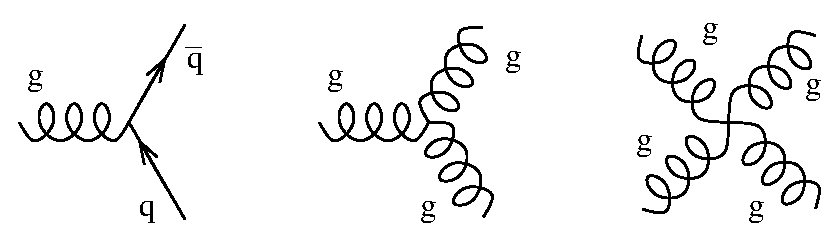
\includegraphics[width=\linewidth]{diagram_qcd}
\end{minipage}

\vfill

\begin{itemize}
  \item It's hard to make quantitative predictions for low-energy
  phenomena, such as spatial wavefunctions, because coupling is too
  strong for a perturbative expansion.
\end{itemize}

\vfill
\begin{minipage}{0.5\linewidth}
  \begin{itemize}
    \item Lattice QCD (LQCD): represent space-time as a 4-D grid of
	quark and gluon field values

    \vspace{1 cm}
    \item Evaluate path integrals as very high-dimensional integral

    \vspace{1 cm}
    \item Computationally intensive
  \end{itemize}
\end{minipage} \hfill \begin{minipage}{0.45\linewidth}
  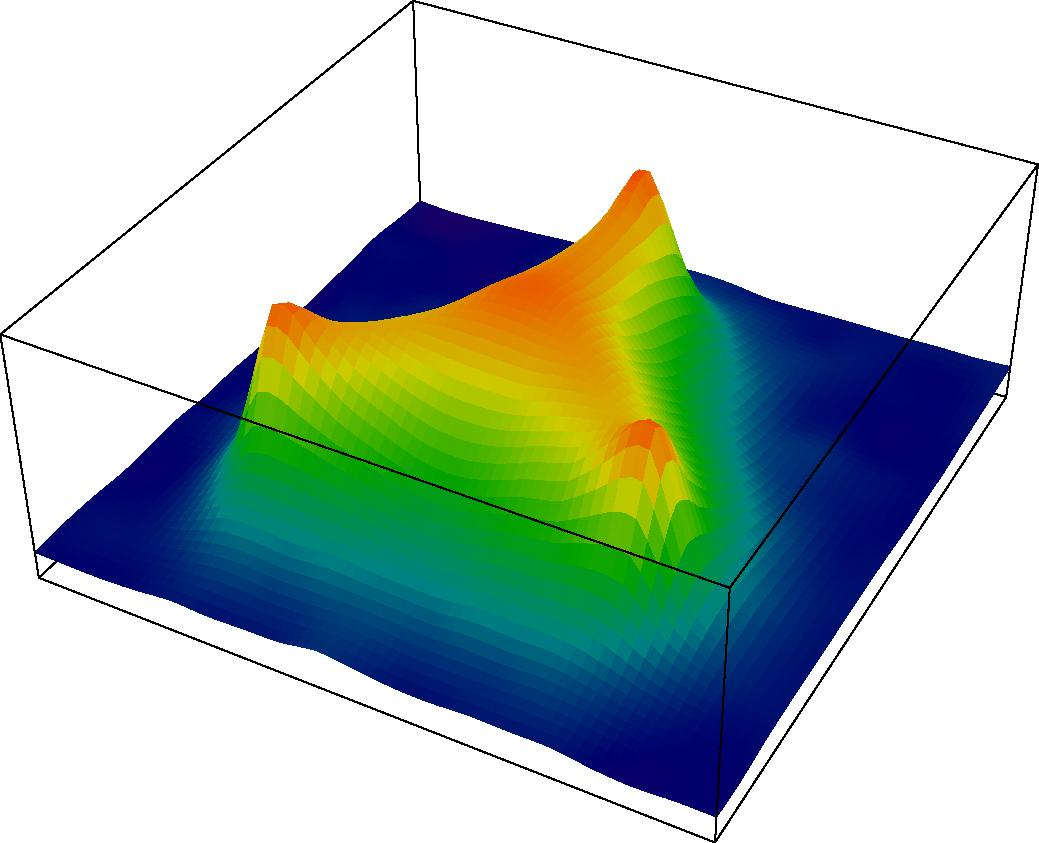
\includegraphics[width=\linewidth]{qcd_proton}
  \begin{center} \large (This is a slice through a proton in action density.) \end{center}
  %% Figures: Recent lattice QCD results for the three-quark flux-tube formation.
  %% [H. Ichie, V. Bornyakov, T. Streuer and G. Schierholz]
\end{minipage}

\end{slide}

\begin{slide}[Precision LQCD: quenched $\to$ unquenched]

\begin{center}
  \begin{tabular}{p{0.35\linewidth} p{0.6\linewidth}}
    \begin{minipage}{\linewidth}
      \begin{center}
	``Quenched'' means ignoring light quark loops ($m_q = \infty$)

	\vspace{1 cm}
	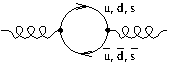
\includegraphics[width=0.75\linewidth]{lqcd_success3}

	\vspace{1 cm}
	``Unquenched'' calculations are made feasible by improved algorithms
      \end{center}
    \end{minipage} &
    \begin{minipage}{\linewidth}
      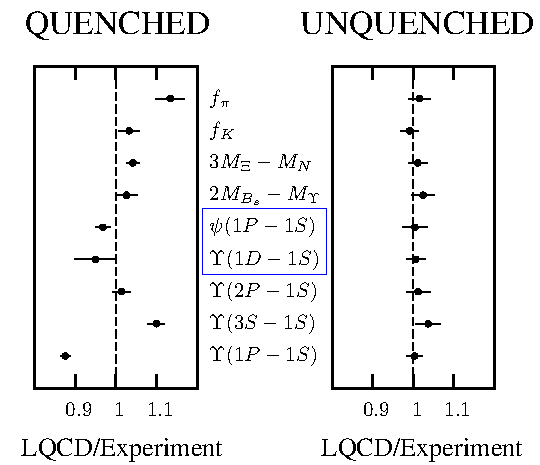
\includegraphics[width=\linewidth]{lqcd_success2}
    \end{minipage}
  \end{tabular}
\end{center}

\vfill Update: $\Omega^-$ and $B_c$ masses also agree with experiment

\vfill CLEO observations of $h_c$ (= $\psi(1P)$) and $\Upsilon(1D)$
were an important part of this program

\end{slide}

%% LQCD for flavor physics: decay rates (1)

%%   * Matrix elements (transition probabilities) instead of eigenvalues
%%     (masses)

%%   * Typically, two particles must meet at a point for the transition
%%     to occur, so this probes fine-grain structure:
%%     |psi(0,0,0)|^2 of spatial wavefunction in real life, lattice
%%     structure in simulation

%%   * The a -> 0 extrapolation is more challenging

\begin{slide}[LQCD for flavor physics: heavy meson decay rates]

\begin{itemize}

  \item Matrix elements (transition probabilities) rather than
  eigenvalues (masses)

  \vfill
  \item Electroweak interactions are point interactions on the scale
  of the spatial wavefunction

  \vfill
  \item Quarks have to find each other: decay rate is governed by
  $|\psi(0,0,0)|^2$

  \begin{center}
    \begin{tabular}{p{6 cm} p{2 cm} p{7 cm} p{3.5 cm}}
      \begin{minipage}{\linewidth}
        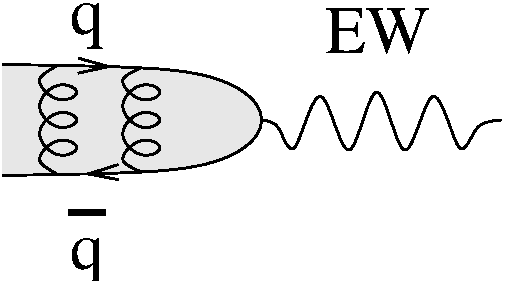
\includegraphics[width=5 cm]{diagram_random}
      \end{minipage} & 
      \begin{minipage}{\linewidth}
        
\includegraphics[height=5 cm]{fuzzytight}
      \end{minipage} & 
      \begin{minipage}{\linewidth}
        yields a faster rate than
      \end{minipage} & 
      \begin{minipage}{\linewidth}
        
\includegraphics[height=5 cm]{fuzzyloose}
      \end{minipage}
    \end{tabular}
  \end{center}

  \vfill
  \color{white} \item Probes fine-grain structure, which is not smooth on the
  lattice

  \vspace{-0.5 cm}
  \begin{center}
    \begin{tabular}{p{6 cm} p{2 cm} p{7 cm} p{3.5 cm}}
      & \begin{minipage}{\linewidth}
        
\includegraphics[height=5 cm]{fuzzytight-white}
      \end{minipage} & 
      \begin{minipage}{\linewidth}
        \mbox{ }
      \end{minipage} & 
      \begin{minipage}{\linewidth}
        
\includegraphics[height=5 cm]{fuzzyloose-white}
      \end{minipage}
    \end{tabular}
  \end{center}
  \vspace{-0.5 cm}

  \vfill
  \item The continuum limit is more challenging for decay rates

\end{itemize}

\end{slide}

\begin{slide}[LQCD for flavor physics: heavy meson decay rates]

\begin{itemize}

  \item Matrix elements (transition probabilities) rather than
  eigenvalues (masses)

  \vfill
  \item Electroweak interactions are point interactions on the scale
  of the spatial wavefunction

  \vfill
  \item Quarks have to find each other: decay rate is governed by
  $|\psi(0,0,0)|^2$

  \begin{center}
    \begin{tabular}{p{6 cm} p{2 cm} p{7 cm} p{3.5 cm}}
      \begin{minipage}{\linewidth}
        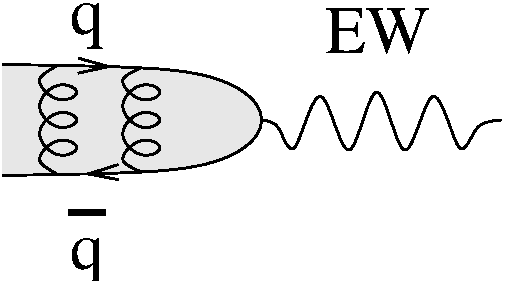
\includegraphics[width=5 cm]{diagram_random}
      \end{minipage} & 
      \begin{minipage}{\linewidth}
        
\includegraphics[height=5 cm]{fuzzytight}
      \end{minipage} & 
      \begin{minipage}{\linewidth}
        yields a faster rate than
      \end{minipage} & 
      \begin{minipage}{\linewidth}
        
\includegraphics[height=5 cm]{fuzzyloose}
      \end{minipage}
    \end{tabular}
  \end{center}

  \vfill
  \item Probes fine-grain structure, which is not smooth on the
  lattice

  \vspace{-0.5 cm}
  \begin{center}
    \begin{tabular}{p{6 cm} p{2 cm} p{7 cm} p{3.5 cm}}
      & \begin{minipage}{\linewidth}
        
\includegraphics[height=5 cm]{fuzzytight-digital}
      \end{minipage} & 
      \begin{minipage}{\linewidth}
        \mbox{ }
      \end{minipage} & 
      \begin{minipage}{\linewidth}
        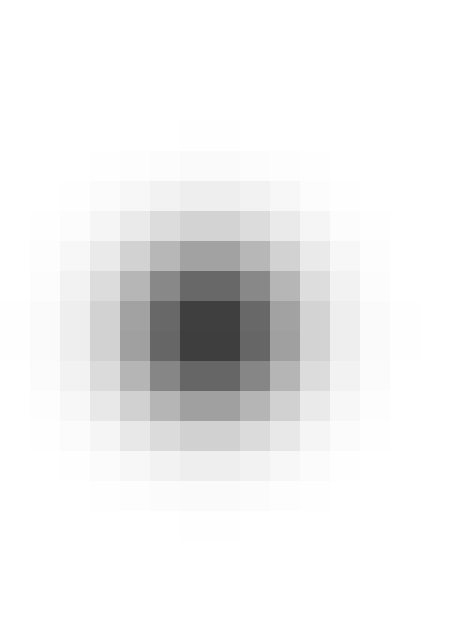
\includegraphics[height=5 cm]{fuzzyloose-digital}
      \end{minipage}
    \end{tabular}
  \end{center}
  \vspace{-0.5 cm}

  \vfill
  \item The continuum limit is more challenging for decay rates

\end{itemize}

\end{slide}

%% Main goal: B meson decay constant (f_B) (1)

%%   * Why?  B\bar{B} mixing could tightly constrain V_td

%%     \Delta m_B = (known) (f_B^2 B_B) |V_td|^2 = 0.502 \pm 0.007 ps^-1 (1.4%)

%%     if QCD factors f_B and B_B could be determined.  (V_td is a CKM
%%     matrix element, a fundumental parameter of SM that constrains CP
%%     asymmetry measurement.)

%%   * If you are familiar with the unitarity triangle, this corresponds
%%     to shrinking the B_d band (20%) to a narrow annulus

%%   * f_B can't be measured directly, as B+ -> l nu rate is too slow to
%%     be observable

%%   * LQCD is the most promising technique for calculating f_B and B_B

\begin{slide}[Main goal: B meson decay constant \boldmath $f_B$]

\begin{minipage}{14 cm} \begin{itemize} \item $B\bar{B}$ mixing could tightly constrain $V_{td}$ \end{itemize} \end{minipage} \hfill \begin{minipage}{10 cm} \begin{center} 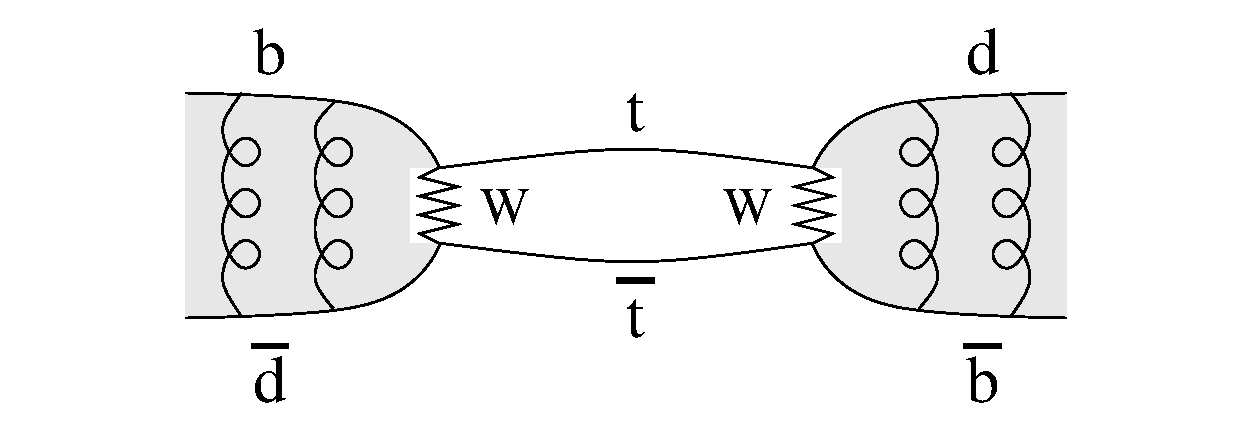
\includegraphics[width=10 cm]{diagram_bmixing} \end{center} \end{minipage}
\[ \Delta M_{B^0,\,\bar{B^0}} = \mbox{(known)} \, {f_B}^2 B_B |V_{td}|^2 = 0.502 \pm 0.007 \mbox{ ps}^{-1} \mbox{ } (1.4\%!) \]

\vspace{0.5 cm}
\mbox{\hspace{0.8 cm}} if QCD factors $f_B$ and $B_B$ could be determined.

\vfill

\begin{minipage}{14 cm}
\color{white} \begin{itemize}
\item Would shrink the 20\% $B_d$ (blue) band to a narrow annulus (few percent)

\vspace{1 cm}

\item $f_B$ and $B_B$ can't be measured directly

\vspace{1 cm}

\item LQCD is the most promising technique for calculating $f_B$ and $B_B$
\end{itemize}
\end{minipage} \hfill \begin{minipage}{10 cm} 
\includegraphics[width=\linewidth]{ckm04-white} \end{minipage}

\end{slide}

\begin{slide}[Main goal: B meson decay constant \boldmath $f_B$]

\begin{minipage}{14 cm} \begin{itemize} \item $B\bar{B}$ mixing could tightly constrain $V_{td}$ \end{itemize} \end{minipage} \hfill \begin{minipage}{10 cm} \begin{center} 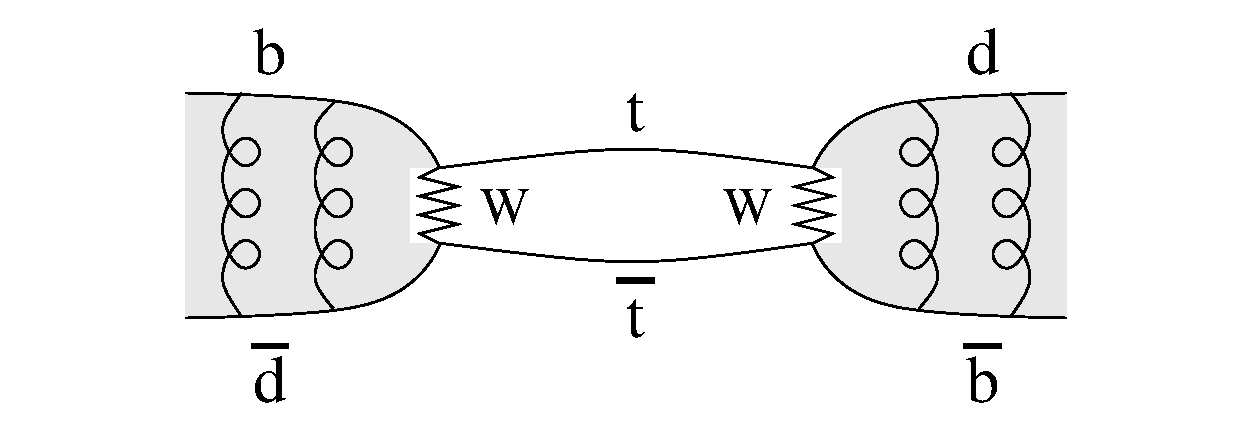
\includegraphics[width=10 cm]{diagram_bmixing} \end{center} \end{minipage}
\[ \Delta M_{B^0,\,\bar{B^0}} = \mbox{(known)} \, {f_B}^2 B_B |V_{td}|^2 = 0.502 \pm 0.007 \mbox{ ps}^{-1} \mbox{ } (1.4\%!) \]

\vspace{0.5 cm}
\mbox{\hspace{0.8 cm}} if QCD factors $f_B$ and $B_B$ could be determined.

\vfill

\begin{minipage}{14 cm}
\begin{itemize}
\item Would shrink the 20\% $B_d$ (blue) band to a narrow annulus (few percent)

\vspace{1 cm}

\item $f_B$ and $B_B$ can't be measured directly

\vspace{1 cm}

\item LQCD is the most promising technique for calculating $f_B$ and $B_B$
\end{itemize}
\end{minipage} \hfill \begin{minipage}{10 cm} 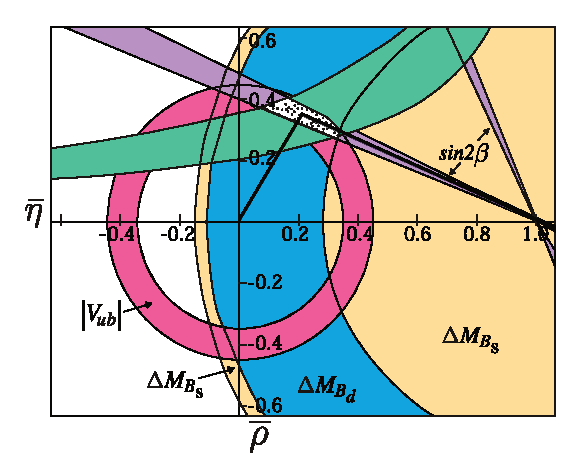
\includegraphics[width=\linewidth]{ckm04} \end{minipage}

\end{slide}

%% The program: LQCD calculates f_B and B_B and predicts related,
%% verifiable quantities (1)

%%              heavy-light    heavy-heavy
%%   * bottom       f_B        \Gamma_ee(U)
%%             (theory only)   (th vs expt)

%%      charm       f_D
%%              (th vs expt)

%%   * Leptonic decays of strongly-bound mesons expose decay constants
%%     (diagrams, label f_D, "f_U", V_cd(known to 1.3%), 1(known))

\begin{slide}[The program: LQCD calculates {\boldmath $f_B$} and related,
verifiable quantities]

\vfill

\vfill

\begin{center}
  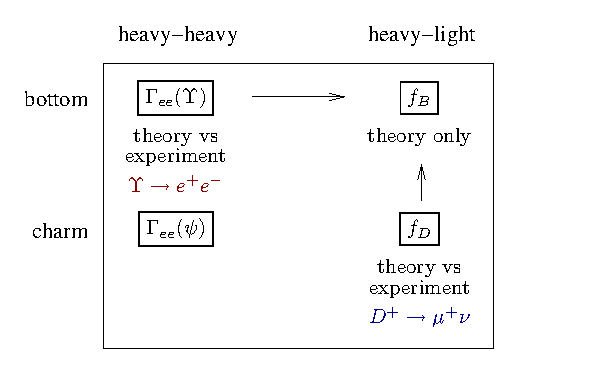
\includegraphics[width=0.7\linewidth]{motivation_table}

  \begin{tabular}{p{0.35\linewidth} p{0.65\linewidth}}
    \begin{minipage}{\linewidth} \begin{center}
	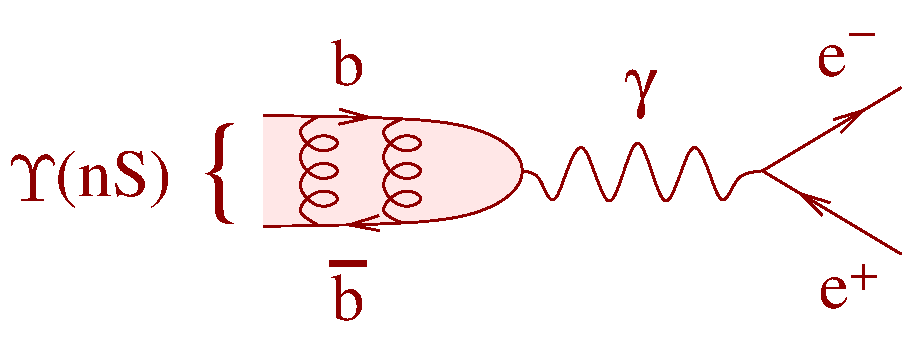
\includegraphics[width=10 cm]{diagram_gamee}
    \end{center} \end{minipage} &
    \begin{minipage}{\linewidth} \begin{center}
	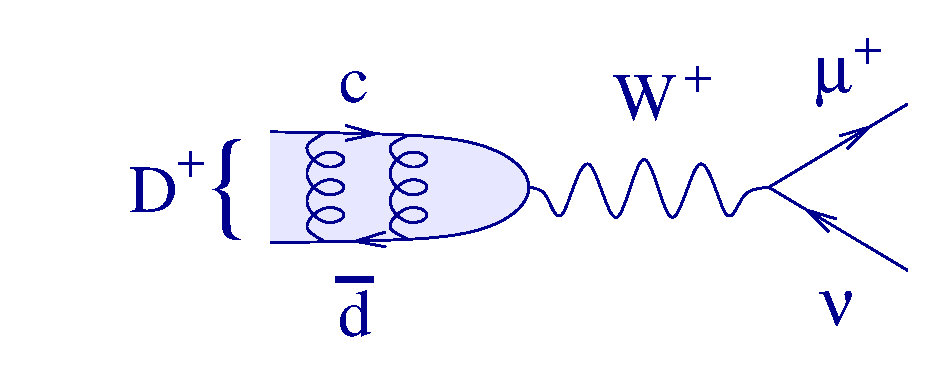
\includegraphics[width=10 cm]{diagram_dtomunu}
    \end{center} \end{minipage} \\
    \begin{minipage}{\linewidth} \[
      \Gamma_{\Upsilon \to e^+e^-} = \frac{16 \pi \, \alpha^2}{3 {M_\Upsilon}^2} \, {\color{dkred} |\psi(0)|^2}
    \] \end{minipage} &
    \begin{minipage}{\linewidth} \[
      \Gamma_{D^+ \to \ell^+\nu} = \frac{{G_F}^2 \, |V_{cd}|^2}{8\pi} {m_\ell}^2 M_D \left(1 - \frac{{m_\ell}^2}{{M_D}^2} \right)^2 {\color{dkblue} {f_D}^2}
    \] \end{minipage}
  \end{tabular}
\end{center}

\end{slide}

%% For the remainder of this talk, I will present (1)

%%   * a high-precision measurement (1.5-2.5%) of \Gamma_ee for
%%     U(1S,2S,3S) (CLEO-III)

%%   * a first statistically-significant observation (6.6 sigma) of D ->
%%     mu nu, which determines f_D to 7.6% (CLEO-c)

%%   * future confrontations between theory and experiment at CLEO-c

\begin{slide}

For the remainder of this talk, I will present

\vspace{1.5 cm}
\begin{itemize}\setlength{\itemsep}{1.5 cm}

  \item a high-precision measurement (1.5--2.5\%) of $\Gamma_{ee}$ for
  $\Upsilon(1S,2S,3S)$ \hfill (15 slides)

  \item observation of 47 $\pm$ 7 $D^+ \to \mu^+ \nu$ events, which
    determines $f_D$ to 7.6\% \hfill (7 slides)

  \item a 4\% measurement of $\Gamma_{ee}$ for $\psi(2S)$ through
    radiative returns \hfill (1 slide)

  \item future confrontations between LQCD and experiment at CLEO-c \hfill (2 slides)

\end{itemize}

\end{slide}

%% GAMMA_EE

%% Roadmap: table of contents and an indicator at the top of the screen (1)

\begin{slidemap}[\mboxy{technique} & \mboxy{backgrounds} & \mboxy{efficiency} & \mboxy{luminosity} & \mboxy{stability} & \mboxy{fits} & \mboxy{results} & \mboxy{theory}]

\begin{center}
  \begin{minipage}{0.7\linewidth}

    $\Gamma_{ee}$ Table of Contents

    \vspace{0.4 cm}
    \begin{center}
      \begin{minipage}{0.95\linewidth}
        \begin{itemize}\setlength{\itemsep}{0.5 cm}

          \item Technique

          \item Backgrounds

          \item Efficiency

          \item Integrated Luminosity

          \item Stability
            \begin{itemize}
              \item Cross-section
              \item Beam energy
            \end{itemize}

          \item Fits

          \item Results

          \item Comparison with theory

        \end{itemize}
      \end{minipage}
    \end{center}

  \end{minipage}

\end{center}

\end{slidemap}

%% Measurement technique I (1)

%%   * By definition, \Gamma_ee(Upsilon) is the decay rate of Upsilon to
%%     e+e- (in absense of other interactions): \Gamma_ee = \Gamma B_ee

%%   * It may seem that a measurement would consist of counting e+e-
%%     final states, but

%%     - this measures B_ee, which is one step removed from \Gamma_ee

%%     - \Gamma can't be measured directly (narrower than collider beam
%%       energy spread)

%%   * Alternative method: time-reversed process (diagrams), measure U
%%     production from e+e- beams (\Gamma_ee = ... \int \sigma dE)

\begin{slidemap}[\mboxy{\color{blue} \bf technique} & \mboxy{backgrounds} & \mboxy{efficiency} & \mboxy{luminosity} & \mboxy{stability} & \mboxy{fits} & \mboxy{results} & \mboxy{theory}]

\vspace{1 cm}
\begin{itemize}\setlength{\itemsep}{0.9 cm}

  \item By definition, $\Gamma_{ee}(\Upsilon)$ is the decay rate of
  $\Upsilon$ to $e^+e^-$ (in absence of other interactions)

\[ \Gamma_{ee} = \Gamma \times \mathcal{B}_{ee} \mbox{ where $\Gamma$ is the resonance width} \]

  \item It may seem that a measurement would consist of counting $e^+e^-$, but

    \vspace{0.2 cm}
    \begin{itemize}\setlength{\itemsep}{0.4 cm}
      \item this measures $\mathcal{B}_{ee}$, which is a step removed
      from $\Gamma_{ee}$

      \item $\Gamma$ can't be measured directly (narrower than
      collider beam energy spread)
    \end{itemize}

  \item Alternative method: consider time-reversed process

  \begin{center}
    \begin{tabular}{p{10 cm} c p{10 cm}}
      \begin{minipage}{\linewidth} \begin{center}
  	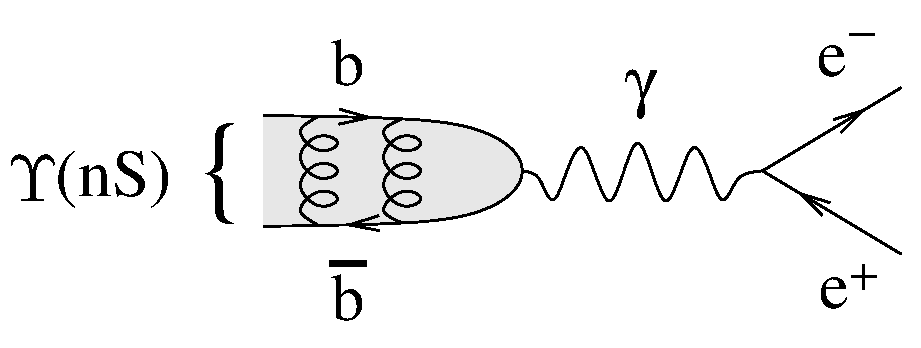
\includegraphics[width=10 cm]{diagram_gamee2}
      \end{center} \end{minipage} & \mbox{\hspace{0.2 cm}} $\to$ \mbox{\hspace{0.2 cm}} &
      \begin{minipage}{\linewidth} \begin{center}
  	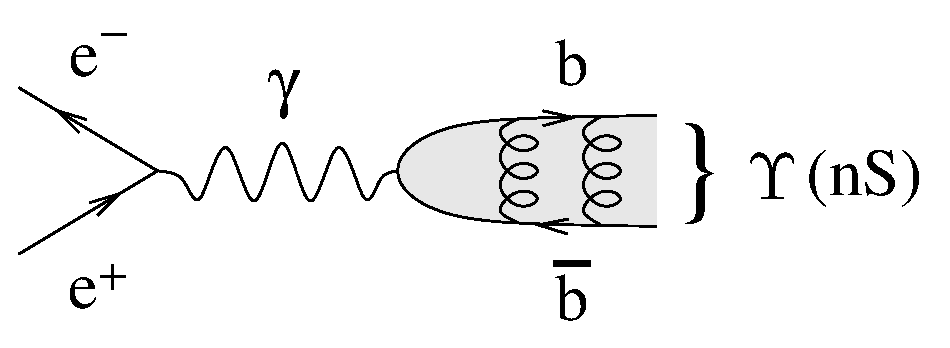
\includegraphics[width=10 cm]{diagram_gamee2-reversed}
      \end{center} \end{minipage}
    \end{tabular}
  \end{center}

  \item Measure $\Upsilon$ {\it production} from $e^+e^-$ beams

\[ \Gamma_{ee} = \frac{{M_\Upsilon}^2}{6 \pi^2} \int \sigma(e^+e^- \to \Upsilon) \, dE \]

\end{itemize}

\end{slidemap}

%% Measurement technique II (3)

%%   * dE integration can be accomplished by scanning U resonance (aerial
%%     view of CESR and cartoon on same slide): cross-section vs. energy

%%   * CLEO-III cut-away; point out silicon, drift chamber, and CsI
%%     calorimeter

%%   * Represent U production with hadronic decays (list cuts)

%%   * U decays to ee, mm, tt: multiply them back in with 1/(1-3 B_mm)
%%     (B_mm precisely measured at CLEO-III (3-4%))

\begin{slidemap}[\mboxy{\color{blue} \bf technique} & \mboxy{backgrounds} & \mboxy{efficiency} & \mboxy{luminosity} & \mboxy{stability} & \mboxy{fits} & \mboxy{results} & \mboxy{theory}]

\begin{itemize}

  \item Scan $\Upsilon$ resonance to perform $dE$ integration

  \item Cross-section versus energy $\to$ integrated cross-section $\to$ $\Gamma_{ee}$

\end{itemize}

\vfill
\begin{center}
  \begin{tabular}{p{0.45\linewidth} c p{0.297\linewidth}}
    \begin{minipage}{\linewidth} \begin{center} Cornell Electron Storage Ring \end{center} \end{minipage} & & \\
    \begin{minipage}{\linewidth}
      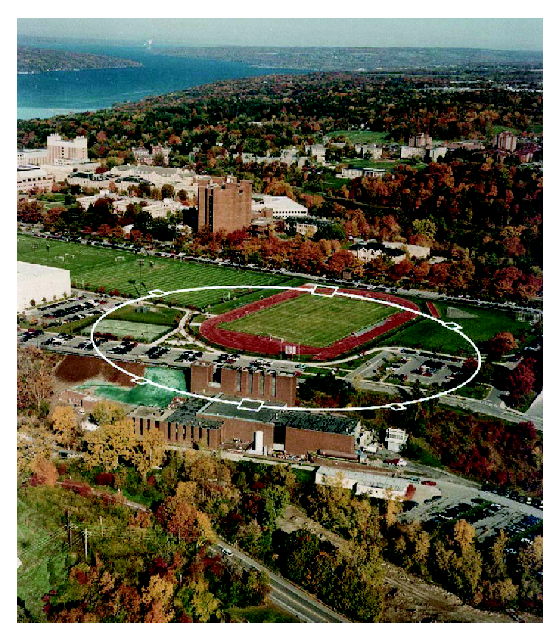
\includegraphics[width=\linewidth]{aerial_200dpi}
    \end{minipage} & \mbox{\hspace{0.6 cm}} &
    \begin{minipage}{\linewidth}
      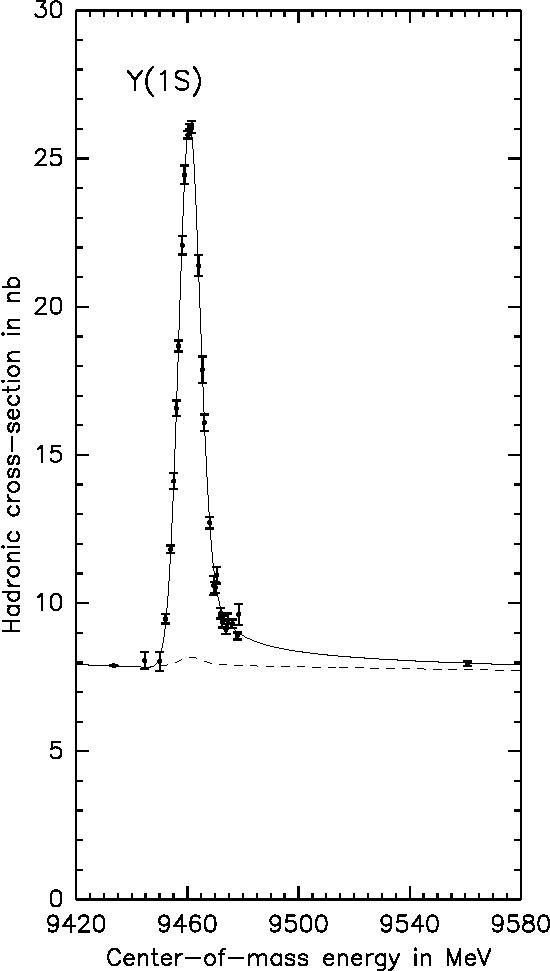
\includegraphics[width=\linewidth]{individual_noinset_1s}
    \end{minipage}
  \end{tabular}
\end{center}

\end{slidemap}

\begin{slidemap}[\mboxy{\color{blue} \bf technique} & \mboxy{backgrounds} & \mboxy{efficiency} & \mboxy{luminosity} & \mboxy{stability} & \mboxy{fits} & \mboxy{results} & \mboxy{theory}]

\begin{center}
  \begin{tabular}{p{0.73\linewidth} p{0.25\linewidth}}
    \begin{minipage}{\linewidth}
      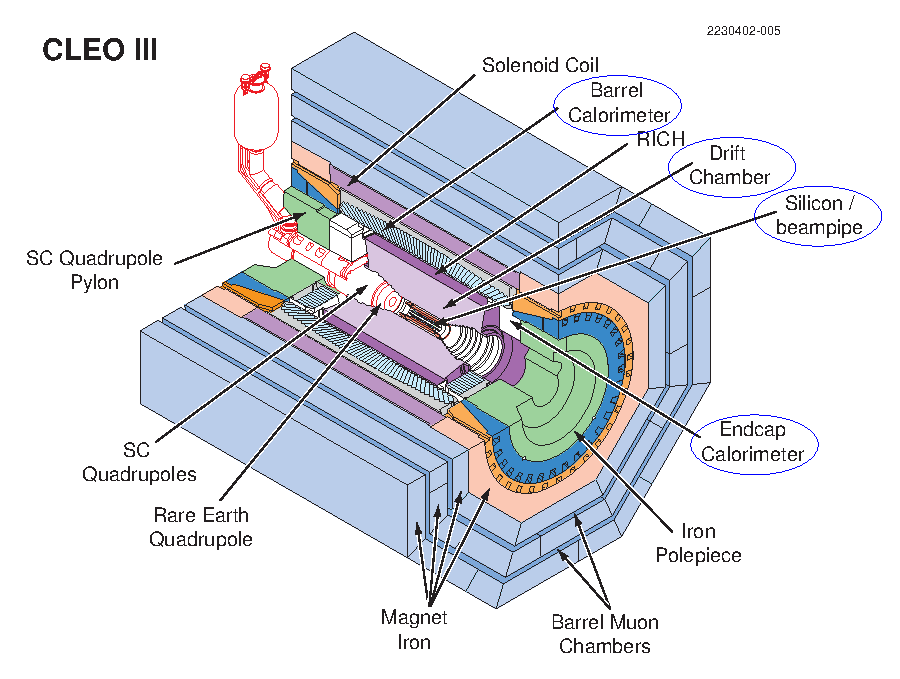
\includegraphics[width=\linewidth]{cleo3_2}
    \end{minipage} &
    \begin{minipage}{\linewidth}
      \begin{tabular}{p{\linewidth}} Event selection \\\hline \end{tabular}
      
      \begin{enumerate}
	\item largest track $|\vec{p}|$ $<$ 80\% $E_{beam}$

	\item observed energy $>$ 40\% $2 \times E_{beam}$

	\item $\exists$ track within 5 mm of beamspot in XY

	\item and within 7.5 cm of beamspot in Z
      \end{enumerate}

    \end{minipage}
  \end{tabular}

\vspace{0.3 cm}

Selection criteria accept only {\it hadronic} decays: total cross-section is
$\displaystyle \sigma_{tot} = \frac{\sigma_{had}}{1 - 3 \mathcal{B}_{\mu\mu}}$

\vspace{0.1 cm}

$\mathcal{B}_{\mu\mu}$ of $\Upsilon(1S,2S,3S)$ measured precisely (3\%, 4\%, 5\%) by CLEO-III

\end{center}

\end{slidemap}

%% Measurement technique III (3)

%%   * Obtain \Gamma_ee from a fit to the resonance lineshape (cartoon)

%%     - Most background processes scale as 1/s

%%     - BW lineshape is convoluted with beam energy spread: does not
%%       affect *area* (== \Gamma_ee)

%%     - Also convoluted with ISR tail (e+e- -> U \gamma) which diverges;
%%       we remove this by

%%       . Constructing a fit function which is BW \otimes G \otimes ISR

%%       . Fitting measured points

%%       . Reading off BW area parameter

%%   * Definition of \Gamma_ee (ee -> U, U -> ee diagrams side-by-side)

%%     - ISR removed             FSR not represented by this measurement

%%     - Vacuum polarization: same in both cases, left in (6% effect)

%%   * Show fits and scan/off lumi for each

%%     - Compare with best lineshapes before CLEO-III

\begin{slidemap}[\mboxy{\color{blue} \bf technique} & \mboxy{backgrounds} & \mboxy{efficiency} & \mboxy{luminosity} & \mboxy{stability} & \mboxy{fits} & \mboxy{results} & \mboxy{theory}]

\vspace{0.25 cm}

\begin{center}
  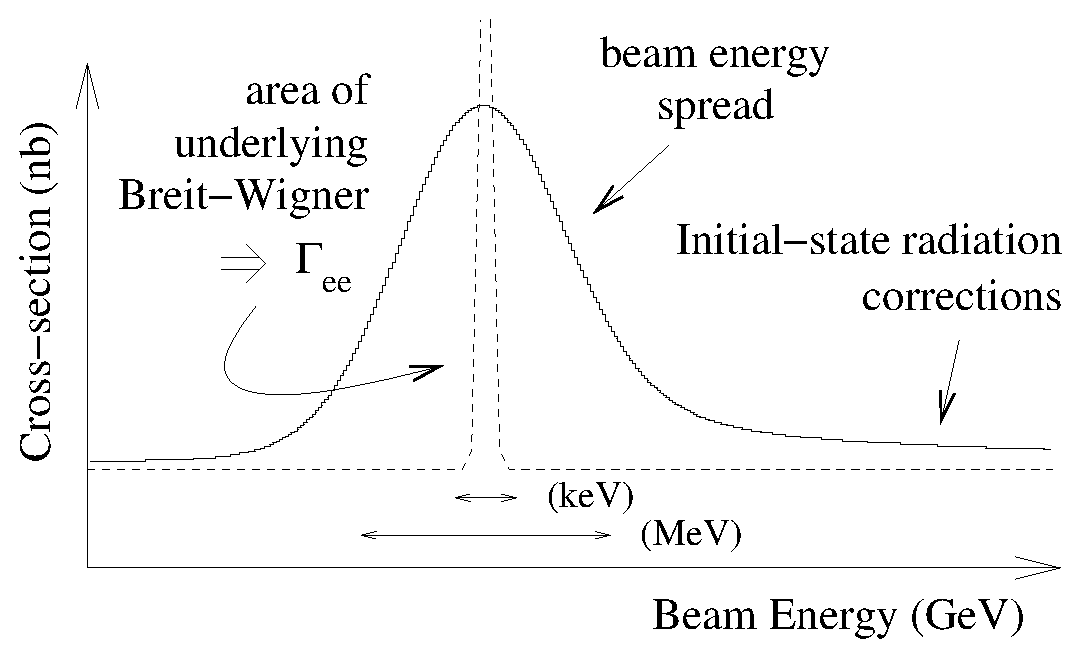
\includegraphics[width=0.6\linewidth]{cartoon}
\end{center}

\begin{itemize}\setlength{\itemsep}{0.5 cm}

  \item Most background processes scale as $1/s$

  \item Breit-Wigner (BW) lineshape is convoluted with beam energy
  spread: \\ does not affect {\it area} (= $\Gamma_{ee}$)

  \item Also convoluted with ISR tail ($e^+e^- \to \gamma \Upsilon$)
  which diverges; we remove this by

  \begin{itemize}\setlength{\itemsep}{0.5 cm}

    \item constructing a fit function which is BW $\otimes$ Gauss $\otimes$ ISR, and

    \item fitting measured points for BW area

  \end{itemize}

\end{itemize}

\end{slidemap}

%% Backgrounds are well-controlled (2)

%%   * Bottom of the sea plot

%%     - Lines are represented in the fit function

%%     - Points are explicitly subtracted, point-by-point

%%   * We explicitly count and subtract cosmic rays and beam-gas

%%     - Single-beam and no-beam samples

%%     - The paper plots: cosmic d_XY is better than beam-gas d_Z

\begin{slidemap}[\mboxy{technique} & \mboxy{\color{blue} \bf backgrounds} & \mboxy{efficiency} & \mboxy{luminosity} & \mboxy{stability} & \mboxy{fits} & \mboxy{results} & \mboxy{theory}]

\vspace{0.5 cm}
\begin{center}
  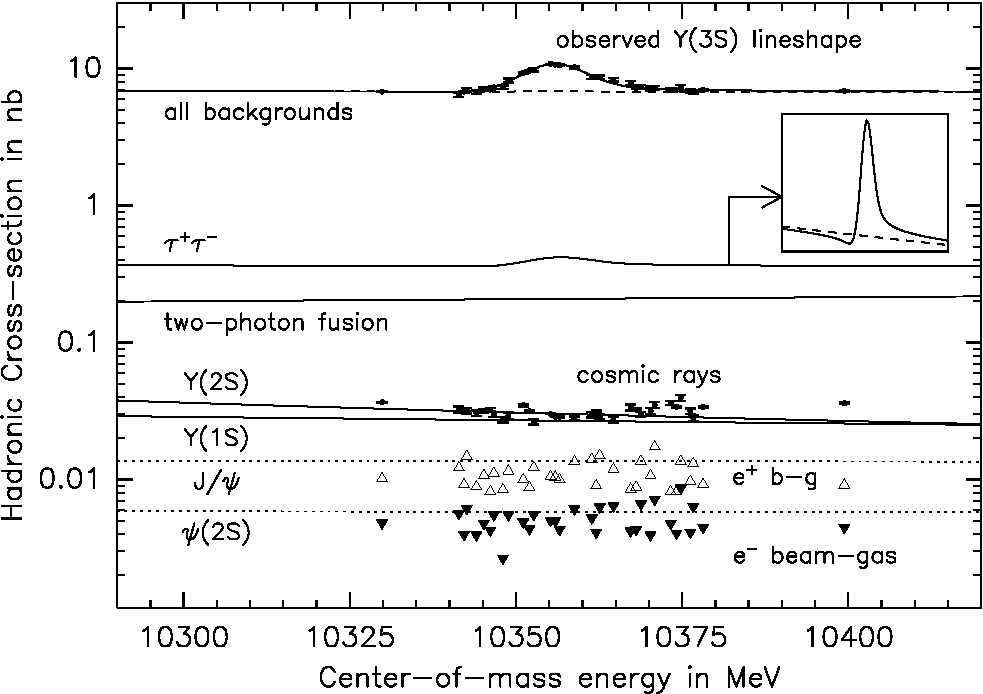
\includegraphics[width=0.8\linewidth]{jed_backgrounds}
\end{center}

\begin{itemize}\setlength{\itemsep}{0.5 cm}

  \item Lines are represented in the fit function

  \item Points (cosmic rays, beam-gas) are explicitly subtracted

\end{itemize}

\end{slidemap}

\begin{slidemap}[\mboxy{technique} & \mboxy{\color{blue} \bf backgrounds} & \mboxy{efficiency} & \mboxy{luminosity} & \mboxy{stability} & \mboxy{fits} & \mboxy{results} & \mboxy{theory}]

\vspace{1 cm}
\begin{center}
  \begin{tabular}{p{0.65\linewidth} c p{0.3\linewidth}}
    \begin{minipage}{\linewidth}
      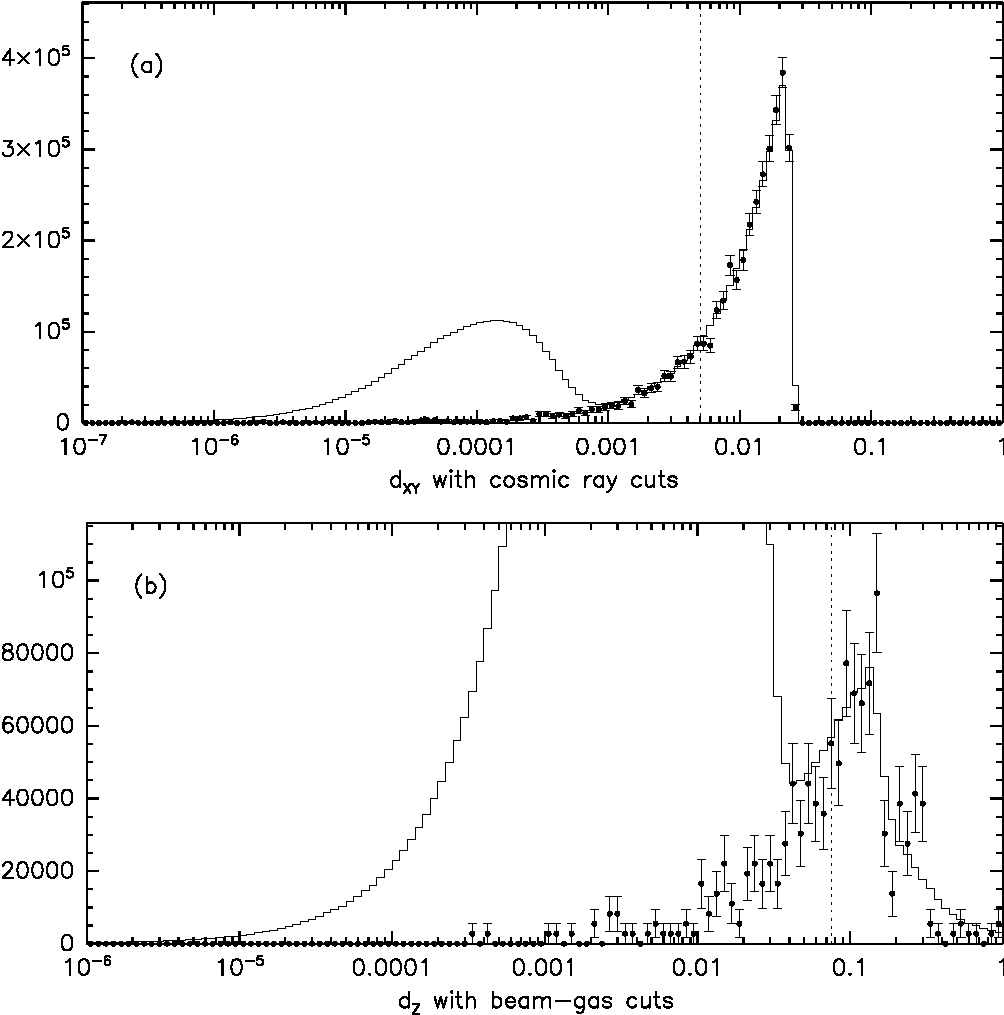
\includegraphics[width=\linewidth]{datasets_database_dxydzcuts}
    \end{minipage} & &
    \begin{minipage}{\linewidth}
      Cosmic rays in scan data (hist) and {\bf no-beam} control sample (points)

      \vspace{6 cm}

      Beam-gas in scan data (hist) and {\bf single-beam} control sample (points)

      \vspace{1 cm}
    \end{minipage}
  \end{tabular}
\end{center}

\end{slidemap}

%% Hadronic efficiency (2)

%%   * Number of U = (U -> hadrons) / (1-3 Bmm)
%%     Hadronic e uncertainty (0.6%) > Bmm e uncertainty (0.2%)

%%   * Want to avoid using MC for hadronic e, as it assumes a
%%     hadronization model

%%   * Model-independent method for measuring hadronic e (1S):

%%     - Select U(2S) -> U(1S) pi+pi- events such that the pi+pi- alone
%%       guarantee inclusion in the dataset (sufficient for trigger)

%%     - Supplies an unbiased set of U(1S) events (includes invisibles
%%       like U -> nu\bar{nu} and even any BSM decays)

%%     - Count (#pass cuts)/(#total) for cut efficiencies

%%     - (Show the recoil mass plots for the unbiased case)

%%     - Efficiency is nearly 100%

%%   * For 2S, 3S hadronic e, most modes are unchanged

%%     - (Use MC for correction factor 1.x +- 0.x consistent with 1)

%%   * Main difference: U(nS) -> X U(n-1S), U(n-1S) -> e+e-, m+m-
%%     have zero efficiency

%%     - Mini-analysis to determine these branching fractions

\begin{slidemap}[\mboxy{technique} & \mboxy{backgrounds} & \mboxy{\color{blue} \bf efficiency} & \mboxy{luminosity} & \mboxy{stability} & \mboxy{fits} & \mboxy{results} & \mboxy{theory}]

\vspace{0.5 cm}
\begin{itemize}\setlength{\itemsep}{0.5 cm}

  \item How many hadronic $\Upsilon$ decays pass event selection?

  \item Model-independent method for measuring $\Upsilon(1S)$ hadronic
    efficiency ($\epsilon_{1S}$):

    \begin{tabular}{p{0.6\linewidth} c p{0.37\linewidth}}
      \begin{minipage}{\linewidth}
	\vspace{1 cm}
        \begin{itemize}\setlength{\itemsep}{0.5 cm}

          \item Select $\Upsilon(2S) \to \pi^+ \pi^- \Upsilon(1S)$
    	    events such that $\pi^+ \pi^-$ alone are sufficient for
    	    event selection

          \item Supplies an unbiased set of $\Upsilon(1S)$ events
    	    (\mbox{includes} invisible decays like $\Upsilon \to
    	    \nu\bar{\nu}$ and Beyond the Standard Model decays)

          \item Count (\#pass event selection)/(\#total)

          \item $\epsilon_{1S}$ is (97.8 $\pm$ 0.5)\%

        \end{itemize}
      \end{minipage} & & \begin{minipage}{\linewidth}
	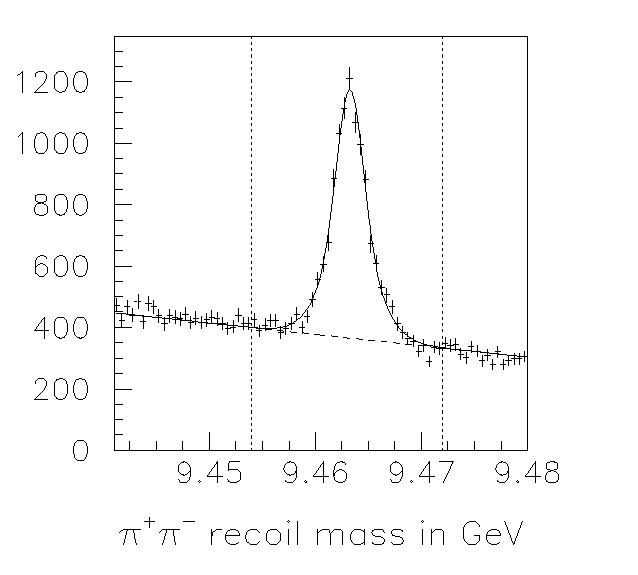
\includegraphics[width=\linewidth]{plenary_justpipimass}
      \end{minipage}
    \end{tabular}

\end{itemize}

\begin{minipage}{0.712\linewidth}
  \color{white} \begin{itemize}\setlength{\itemsep}{0.5 cm}

    \item For $\epsilon_{2S}$, $\epsilon_{3S}$, most modes are unchanged

    \item $\Upsilon(nS) \to X \Upsilon$ where $\Upsilon \to e^+e^-$, $\mu^+\mu^-$ have zero efficiency
    
    \item Mini-analysis to determine these branching fractions in data

  \end{itemize}
\end{minipage} \begin{minipage}{0.25\linewidth}
  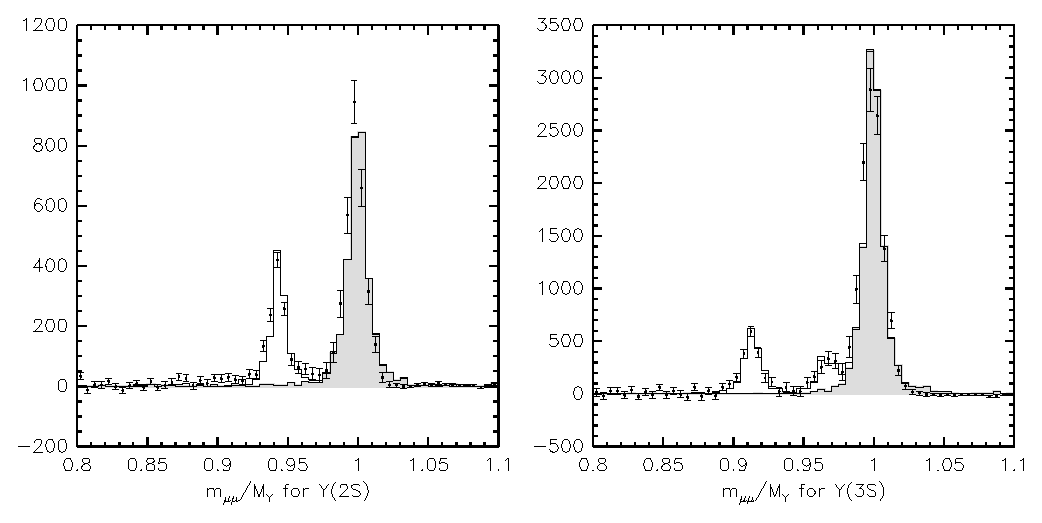
\includegraphics[width=\linewidth, viewport=245 500 490 740, clip=true]{beautiful_bcasll_2}
\end{minipage}

\end{slidemap}

\begin{slidemap}[\mboxy{technique} & \mboxy{backgrounds} & \mboxy{\color{blue} \bf efficiency} & \mboxy{luminosity} & \mboxy{stability} & \mboxy{fits} & \mboxy{results} & \mboxy{theory}]

\vspace{0.5 cm}
\begin{itemize}\setlength{\itemsep}{0.5 cm}

  \item How many hadronic $\Upsilon$ decays pass event selection?

  \item Model-independent method for measuring $\Upsilon(1S)$ hadronic
    efficiency ($\epsilon_{1S}$):

    \begin{tabular}{p{0.6\linewidth} c p{0.37\linewidth}}
      \begin{minipage}{\linewidth}
	\vspace{1 cm}
        \begin{itemize}\setlength{\itemsep}{0.5 cm}

          \item Select $\Upsilon(2S) \to \pi^+ \pi^- \Upsilon(1S)$
    	    events such that $\pi^+ \pi^-$ alone are sufficient for
    	    event selection

          \item Supplies an unbiased set of $\Upsilon(1S)$ events
    	    (\mbox{includes} invisible decays like $\Upsilon \to
    	    \nu\bar{\nu}$ and Beyond the Standard Model decays)

          \item Count (\#pass event selection)/(\#total)

          \item $\epsilon_{1S}$ is (97.8 $\pm$ 0.5)\%

        \end{itemize}
      \end{minipage} & & \begin{minipage}{\linewidth}
	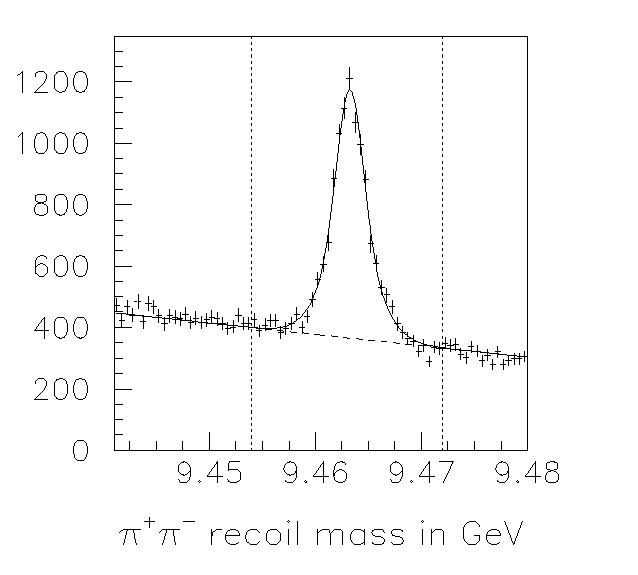
\includegraphics[width=\linewidth]{plenary_justpipimass}
      \end{minipage}
    \end{tabular}

\end{itemize}

\begin{minipage}{0.712\linewidth}
  \begin{itemize}\setlength{\itemsep}{0.5 cm}

    \item For $\epsilon_{2S}$, $\epsilon_{3S}$, most modes are unchanged

    \item $\Upsilon(nS) \to X \Upsilon$ where $\Upsilon \to e^+e^-$, $\mu^+\mu^-$ have zero efficiency
    
    \item Mini-analysis to determine these branching fractions in data

  \end{itemize}
\end{minipage} \begin{minipage}{0.25\linewidth}
  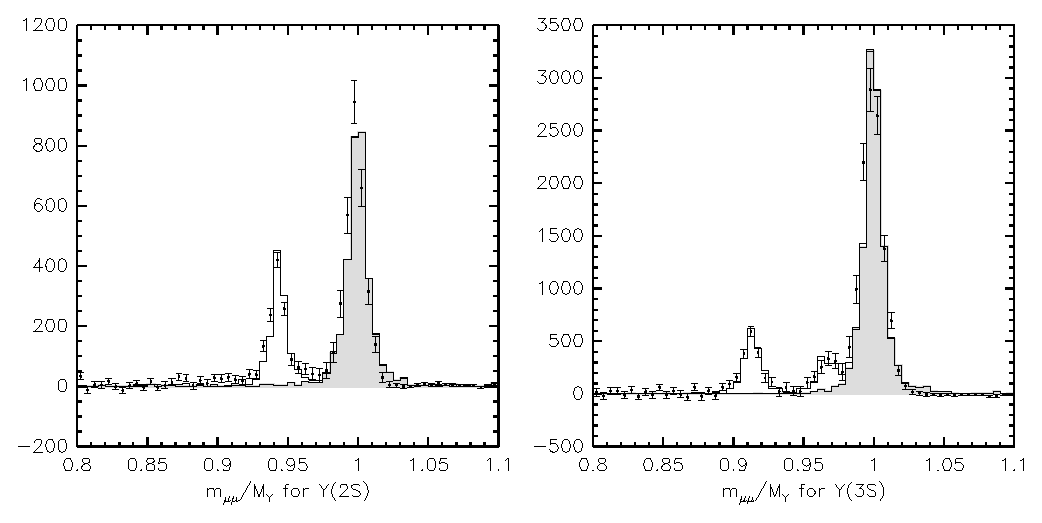
\includegraphics[width=\linewidth, viewport=245 0 490 240, clip=true]{beautiful_bcasll_2}
\end{minipage}

\end{slidemap}

%% Integrated Luminosity (1)

%%   * Need to know integrated luminosity (amount of data) for each scan
%%     point

%%   * Divide problem into relative int lumis (determine all up to a
%%     single constant) and absolute int lumi (determine the last
%%     constant)

%%   * Relative int lumis:

%%     - Count #e+e- -> \gamma\gamma at each scan point

%%     - Int lumi is proportional to #\gamma\gamma * beam energy^2

%%     - This is enough to plot cross-section vs energy, with
%%       cross-section in unknown units

%%   * Absolute int lumis:

%%     - Separate analysis involving e+e-, \gamma\gamma, m+m- final
%%       states

%%     - Blinded \Gamma_ee analysis by applying this correction at the
%%       very end

\begin{slidemap}[\mboxy{technique} & \mboxy{backgrounds} & \mboxy{efficiency} & \mboxy{\color{blue} \bf luminosity} & \mboxy{stability} & \mboxy{fits} & \mboxy{results} & \mboxy{theory}]

\begin{itemize}\setlength{\itemsep}{0.75 cm}

  \item Need to know integrated luminosity for each scan point

  \item Int lumi for a point relative to other scan points:

  \vspace{0.5 cm}
  \begin{itemize}\setlength{\itemsep}{0.75 cm}

    \item Int lumi $\propto$ (\#$e^+e^- \to \gamma\gamma$) $\times$ ${E_{beam}}^2$

    \item This is enough to do fits, with cross-section in unknown
      units

  \end{itemize}

\end{itemize}

\vspace{1 cm}
\begin{minipage}{0.45\linewidth}
  \begin{itemize}\setlength{\itemsep}{0.75 cm}

    \item Determine overall scale for int lumi:

      \vspace{0.5 cm}
      \begin{itemize}\setlength{\itemsep}{0.75 cm}

        \item Separate analysis involving $e^+e^-$, $\gamma\gamma$, and
	  $\mu^+\mu^-$ final states

	\item Blinded $\Gamma_{ee}$ analysis by applying this correction
	  at the end

	  \vspace{3 cm}

      \end{itemize}

  \end{itemize}
\end{minipage} \mbox{\hspace{0.05\linewidth}} \begin{minipage}{0.5\linewidth}
  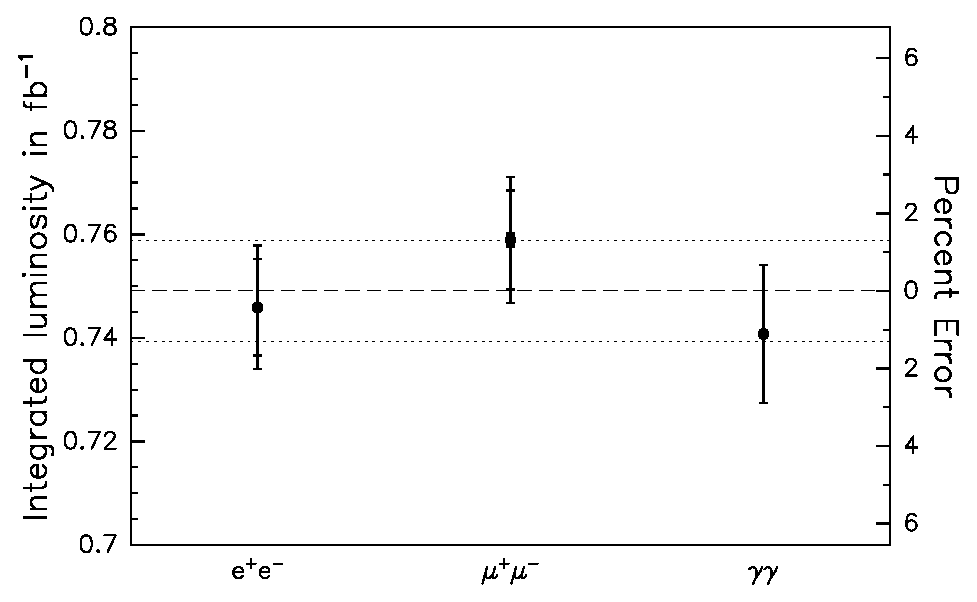
\includegraphics[width=\linewidth]{plenary_lumi}
\end{minipage}

\end{slidemap}

%% Cross-section stability (1)

%%   * 500 measurements of cross-section (below resonance) are consistent
%%     with a single value

%%     - Pull distributions are unit Gaussians

%%     - Same is true if relative int lumit is measured by Bhabhas

%%     - This is a larger sample of data than the scan

\begin{slidemap}[\mboxy{technique} & \mboxy{backgrounds} & \mboxy{efficiency} & \mboxy{luminosity} & \mboxy{\color{blue} \bf stability} & \mboxy{fits} & \mboxy{results} & \mboxy{theory}]

  \vspace{1.5 cm}
  \begin{center}
    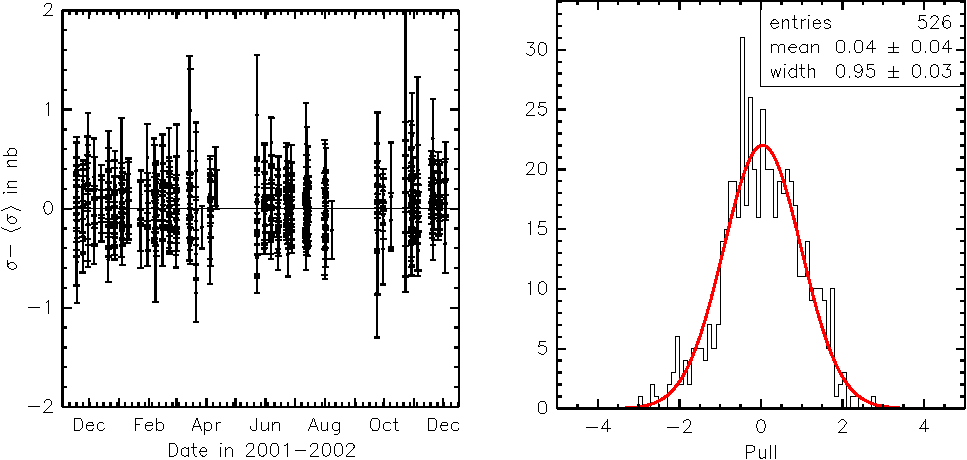
\includegraphics[width=0.95\linewidth]{stability}
  \end{center}

  \vspace{0.5 cm}
  \begin{itemize}\setlength{\itemsep}{0.75 cm}

    \item All off-resonance runs at a given energy reproduce the same
      cross-section

    \item Cross-section {\bf in}stability $\lesssim$ 0.03 nb

  \end{itemize}

\end{slidemap}

%% Beam-energy measurement stability (2, really 1)

%%   * Weekly scans were short and independent

%%   * Measurements alternated above and below resonance peak

%%   * Point of high slope was repeated in the scan

%%     - Energy measurement stability from consistency of that repeated
%%       point

%%     - 30 measurements, consistent with zero, yield upper limit of 0.07
%%       MeV

\begin{slidemap}[\mboxy{technique} & \mboxy{backgrounds} & \mboxy{efficiency} & \mboxy{luminosity} & \mboxy{\color{blue} \bf stability} & \mboxy{fits} & \mboxy{results} & \mboxy{theory}]

  \begin{tabular}{p{0.6\linewidth} p{0.38\linewidth}}
    \begin{minipage}{\linewidth}
      \begin{minipage}{0.9\linewidth}
	\begin{itemize}
          \item weekly scans were short and independent
          \item measurements alternated above and below \mbox{resonance} peak
          \item a point of high slope was repeated in the scan
	\end{itemize}
      \end{minipage}

      \vspace{0.5 cm}
      \begin{center}
        
\includegraphics[width=0.95\linewidth]{proceedings_miscal_white}

        \vspace{1 cm}
        \textcolor{white}{Beam-energy {\bf in}stability $\lesssim$ 0.07 MeV}
      \end{center}

    \end{minipage} &
    \begin{minipage}{\linewidth}
      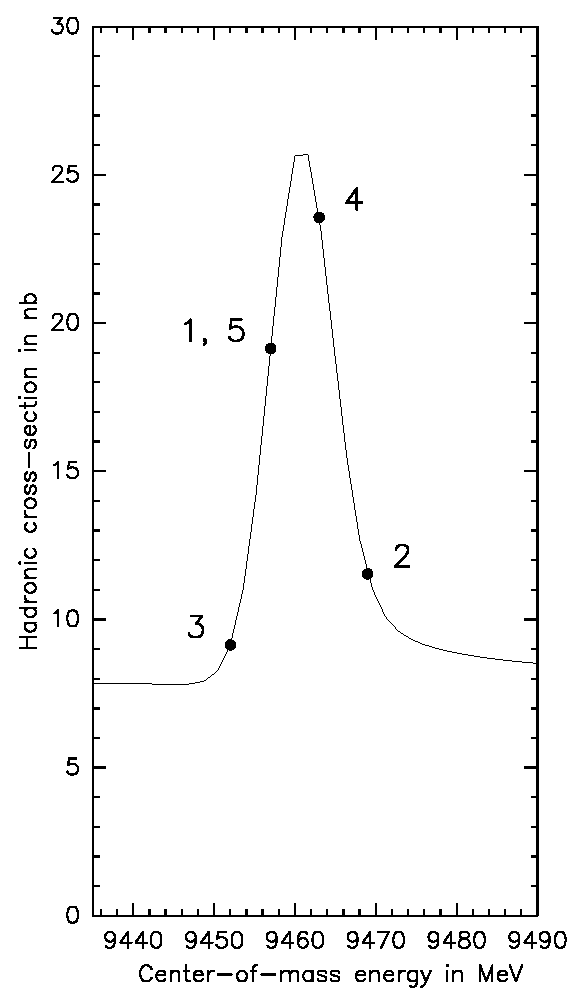
\includegraphics[width=\linewidth]{plenary_fitorder}
    \end{minipage}
  \end{tabular}

\end{slidemap}

\begin{slidemap}[\mboxy{technique} & \mboxy{backgrounds} & \mboxy{efficiency} & \mboxy{luminosity} & \mboxy{\color{blue} \bf stability} & \mboxy{fits} & \mboxy{results} & \mboxy{theory}]

  \begin{tabular}{p{0.6\linewidth} p{0.38\linewidth}}
    \begin{minipage}{\linewidth}
      \begin{minipage}{0.9\linewidth}
	\begin{itemize}
          \item weekly scans were short and independent
          \item measurements alternated above and below \mbox{resonance} peak
          \item a point of high slope was repeated in the scan
	\end{itemize}
      \end{minipage}

      \vspace{0.5 cm}
      \begin{center}
        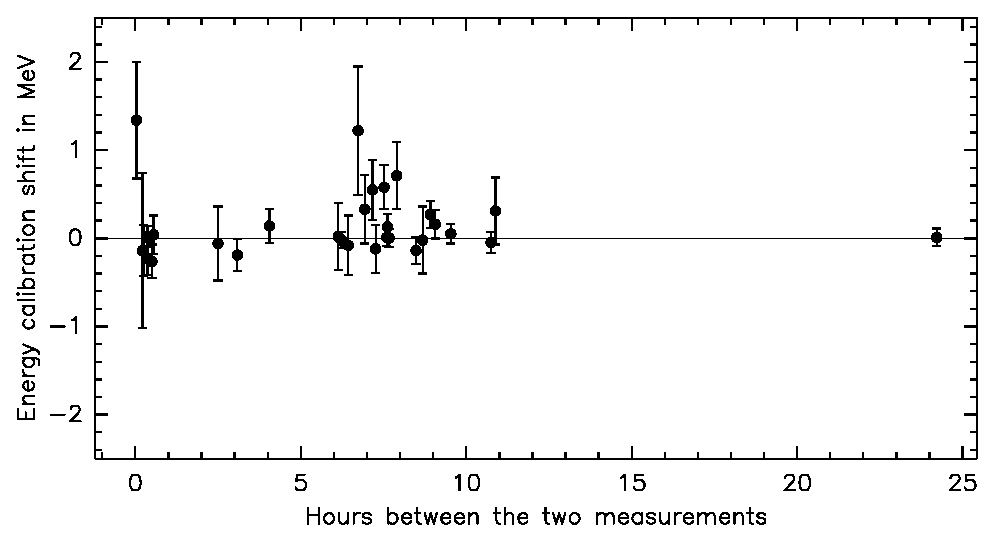
\includegraphics[width=0.95\linewidth]{proceedings_miscal}

        \vspace{1 cm}
        Beam-energy {\bf in}stability $\lesssim$ 0.07 MeV
      \end{center}

    \end{minipage} &
    \begin{minipage}{\linewidth}
      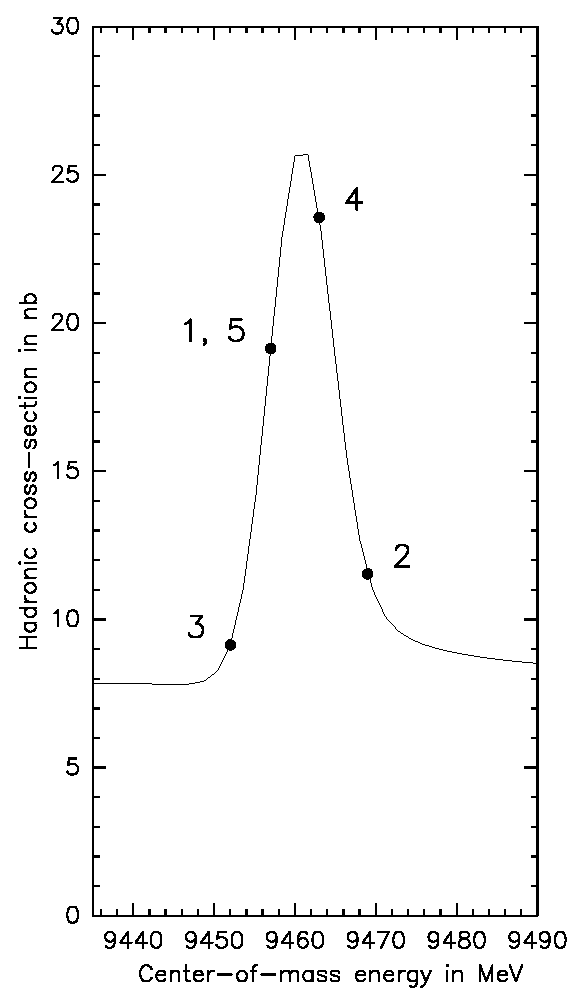
\includegraphics[width=\linewidth]{plenary_fitorder}
    \end{minipage}
  \end{tabular}

\end{slidemap}

%% Fit results (just like last talk) (4, really 2)

\begin{slidemap}[\mboxy{technique} & \mboxy{backgrounds} & \mboxy{efficiency} & \mboxy{luminosity} & \mboxy{stability} & \mboxy{\color{blue} \bf fits} & \mboxy{results} & \mboxy{theory}]

\begin{tabular}{p{0.6\linewidth} p{0.38\linewidth}}
  \begin{minipage}{\linewidth}
    {\bf Parameters:}

    \vspace{0.75 cm}
    \mbox{\hspace{1 cm}} \begin{minipage}{0.85\linewidth}
      \begin{enumerate}\setlength{\itemsep}{0.5 cm}
        \item Area without tail (MeV nb) $\longrightarrow$ $\Gamma_{ee}$ (keV)
        \item Beam energy spread (MeV)
        \item Background level (nb)
          \renewcommand{\labelenumi}{4--15.}
        \item Upsilon mass for each weekly scan (MeV)
      \end{enumerate}
    \end{minipage}

    \vspace{1 cm}
    {\bf Fit function:}

    \vspace{0.75 cm}
    \mbox{\hspace{1 cm}} \begin{minipage}{0.85\linewidth}
      \begin{enumerate}\setlength{\itemsep}{0.75 cm}
        \item Breit-Wigner $\otimes$ Gaussian $\otimes$ ISR tail \\
          (Kuraev and Fadin 0.1\% calculation)
          
          Includes interference term (small effect)
        \item $\tau^+\tau^-$ background peaks under signal, \\
          precisely subtracted with CLEO-III $\mathcal{B}_{\tau\tau}$
        \item Smooth backgrounds: $1/s$, $\log s$, ISR tails
      \end{enumerate}
    \end{minipage}
  \end{minipage} &
  \begin{minipage}{\linewidth}
    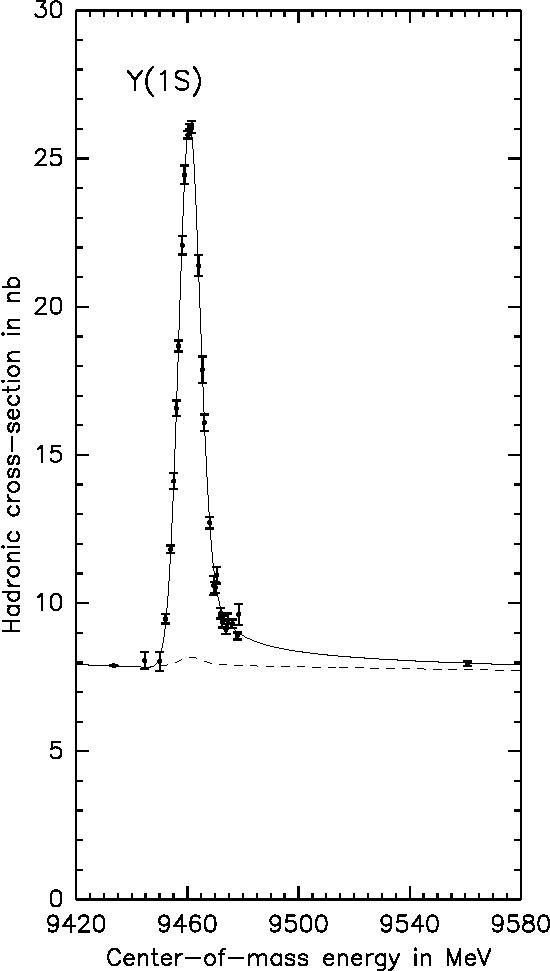
\includegraphics[width=\linewidth]{individual_noinset_1s}
  \end{minipage}
\end{tabular}

\end{slidemap}

\begin{slidemap}[\mboxy{technique} & \mboxy{backgrounds} & \mboxy{efficiency} & \mboxy{luminosity} & \mboxy{stability} & \mboxy{\color{blue} \bf fits} & \mboxy{results} & \mboxy{theory}]

\begin{center}
  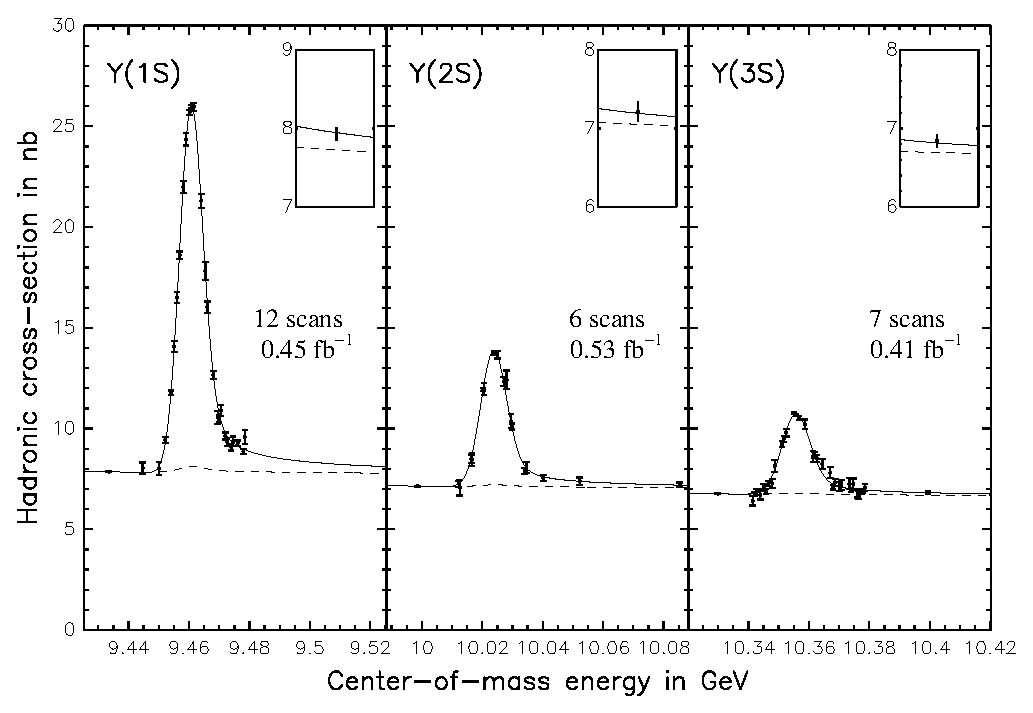
\includegraphics[width=\linewidth]{three_resonances_inset_squat2_nscans}
\end{center}

\end{slidemap}

\begin{slidemap}[\mboxy{technique} & \mboxy{backgrounds} & \mboxy{efficiency} & \mboxy{luminosity} & \mboxy{stability} & \mboxy{\color{blue} \bf fits} & \mboxy{results} & \mboxy{theory}]

  \begin{center}
    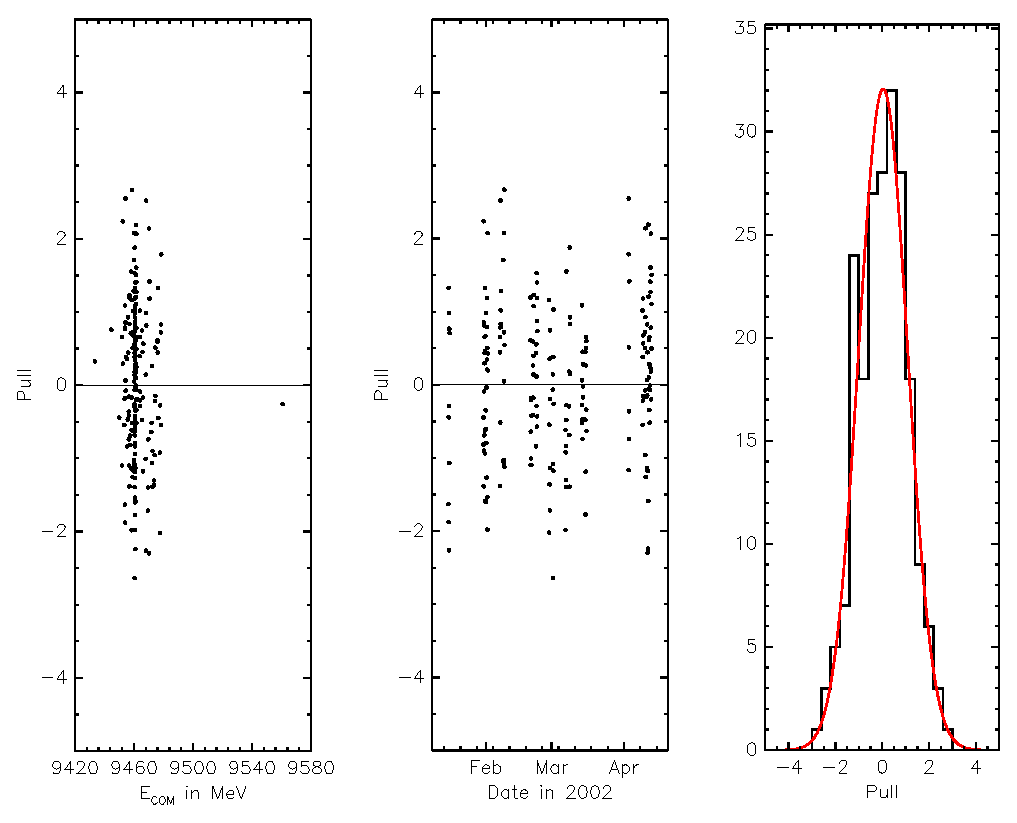
\includegraphics[width=0.81\linewidth]{plenary_pulls1}
  \end{center}
  $\Upsilon(1S)$ Pull Distributions: $\chi^2/$ndf = 230/195 = 1.2, C.L. = 4\%
\end{slidemap}

\begin{slidemap}[\mboxy{technique} & \mboxy{backgrounds} & \mboxy{efficiency} & \mboxy{luminosity} & \mboxy{stability} & \mboxy{\color{blue} \bf fits} & \mboxy{results} & \mboxy{theory}]

  \begin{center}
    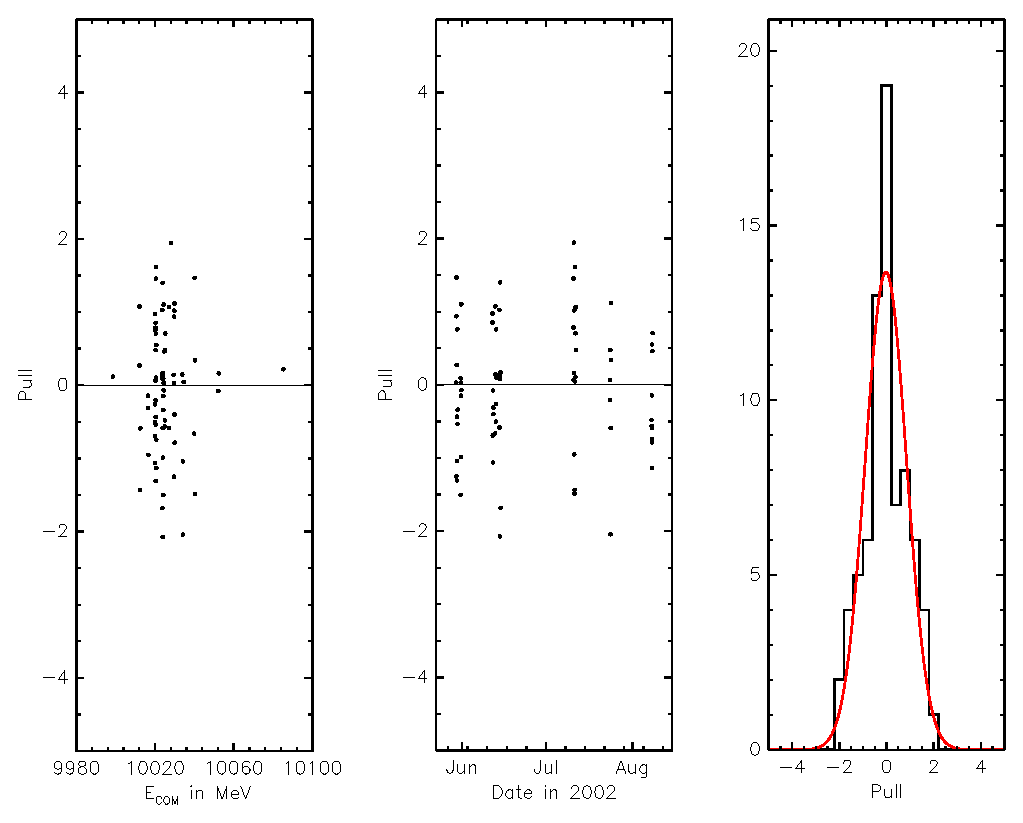
\includegraphics[width=0.81\linewidth]{plenary_pulls2}
  \end{center}
  $\Upsilon(2S)$ Pull Distributions: $\chi^2/$ndf = 58/66 = 0.87, C.L. = 76\%
\end{slidemap}

\begin{slidemap}[\mboxy{technique} & \mboxy{backgrounds} & \mboxy{efficiency} & \mboxy{luminosity} & \mboxy{stability} & \mboxy{\color{blue} \bf fits} & \mboxy{results} & \mboxy{theory}]

  \begin{center}
    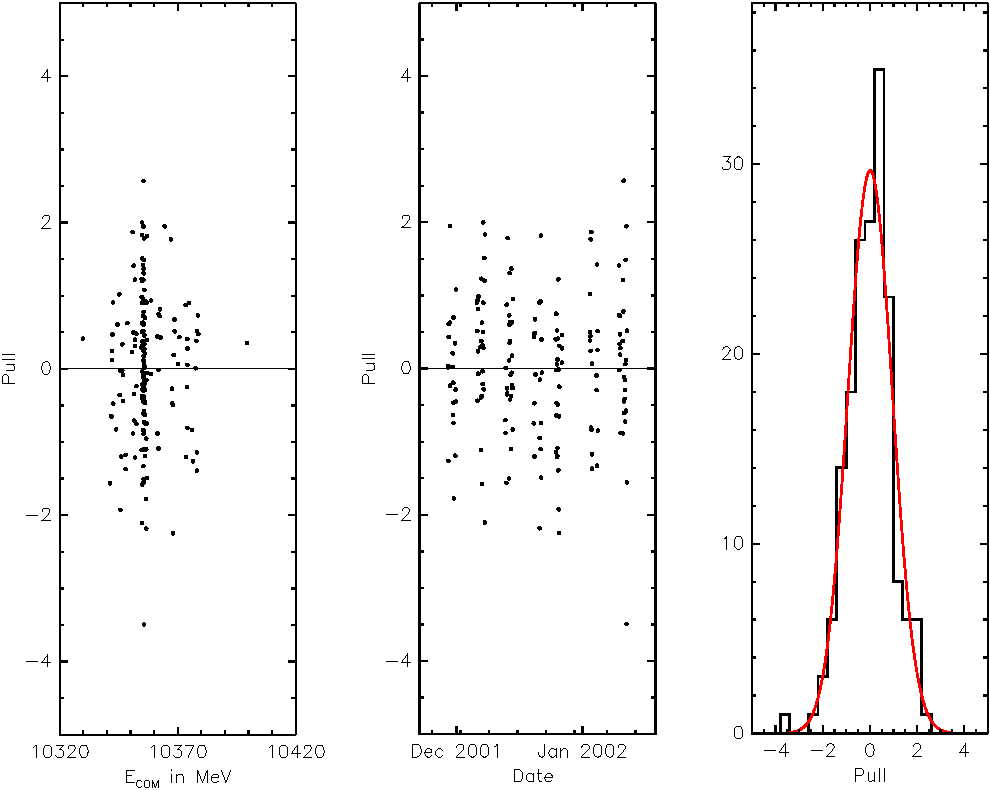
\includegraphics[width=0.81\linewidth]{plenary_pulls3}
  \end{center}
  $\Upsilon(3S)$ Pull Distributions: $\chi^2/$ndf = 155/165 = 0.94, C.L. = 70\%
\end{slidemap}

%% Summary of uncertainties (just like last talk) (1)

\begin{slidemap}[\mboxy{technique} & \mboxy{backgrounds} & \mboxy{efficiency} & \mboxy{luminosity} & \mboxy{stability} & \mboxy{fits} & \mboxy{\color{blue} \bf results} & \mboxy{theory}]

  \vspace{1 cm}
  {\bf Summary of Uncertainties}
  \begin{center}
    \renewcommand{\arraystretch}{1.25}
    \begin{tabular}{l c c c}
      Contribution to $\Gamma_{ee}$ & \mbox{\hspace{1 cm}} $\Upsilon(1S)$ \mbox{\hspace{1 cm}} & \mbox{\hspace{1 cm}} $\Upsilon(2S)$ \mbox{\hspace{1 cm}} & \mbox{\hspace{1 cm}} $\Upsilon(3S)$ \mbox{\hspace{1 cm}} \\\hline
      Statistical$^*$               & {\bf 0.7\%}  & {\bf 1.6\%}  & {\bf 2.2\%} \\
      $(1 - 3\mathcal{B}_{\mu\mu})$ & 0.2\%  & 0.2\%  & 0.3\% \\
      Hadronic efficiency           & 0.5\%  & 0.6\%  & 0.7\% \\
      Luminosity calibration        & {\bf 1.3\%}  & {\bf 1.3\%}  & {\bf 1.3\%} \\
      Cross-section stability       & 0.1\%  & 0.1\%  & 0.1\% \\
      Beam-energy stability         & 0.2\%  & 0.2\%  & 0.2\% \\
      Shape of the fit function     & 0.05\% & 0.06\% & 0.05\% \\\hline
      Total                         & {\bf 1.6\%}  & {\bf 2.2\%}  & {\bf 2.7\%} \\
    \end{tabular}
  \end{center}

  \vspace{1 cm}
  \mbox{ }$^*$\begin{minipage}{0.9\linewidth}

    \vspace{1 cm}
    Statistical uncertainty is dominated by run-by-run luminosity
    measurement ($e^+e^- \to \gamma\gamma$ counting) and contains
    background subtractions.
  \end{minipage}
\end{slidemap}

%% Preliminary results (just like last talk, with PDG plots) (2)

\begin{slidemap}[\mboxy{technique} & \mboxy{backgrounds} & \mboxy{efficiency} & \mboxy{luminosity} & \mboxy{stability} & \mboxy{fits} & \mboxy{\color{blue} \bf results} & \mboxy{theory}]

  \vspace{1 cm}
  {\bf Preliminary Results}
  \begin{center}
    \renewcommand{\arraystretch}{2}
    \begin{tabular}{c c c}
      Quantity & Value & \mbox{\hspace{0.5 cm}} Uncertainty \mbox{\hspace{0.5 cm}} \\ \hline
      $\Gamma_{ee}(1S)$ & \mbox{\hspace{0.5 cm}} 1.336 $\pm$ 0.009 $\pm$ 0.019 keV \mbox{\hspace{0.5 cm}} & 1.6\% \\
      $\Gamma_{ee}(2S)$ & 0.616 $\pm$ 0.010 $\pm$ 0.009 keV & 2.2\% \\
      $\Gamma_{ee}(3S)$ & 0.425 $\pm$ 0.009 $\pm$ 0.006 keV & 2.7\% \\ \hline
      $\Gamma_{ee}(2S)$/$\Gamma_{ee}(1S)$ & 0.461 $\pm$ 0.008 $\pm$ 0.003 & 1.8\% \\
      $\Gamma_{ee}(3S)$/$\Gamma_{ee}(1S)$ & 0.318 $\pm$ 0.007 $\pm$ 0.002 & 2.4\% \\
      $\Gamma_{ee}(3S)$/$\Gamma_{ee}(2S)$ & 0.690 $\pm$ 0.019 $\pm$ 0.006 & 2.8\% \\
    \end{tabular}
  \end{center}

  \vfill
  Presented at EPS, Lattice05
\end{slidemap}

\begin{slidemap}[\mboxy{technique} & \mboxy{backgrounds} & \mboxy{efficiency} & \mboxy{luminosity} & \mboxy{stability} & \mboxy{fits} & \mboxy{\color{blue} \bf results} & \mboxy{theory}]

  \begin{center}
    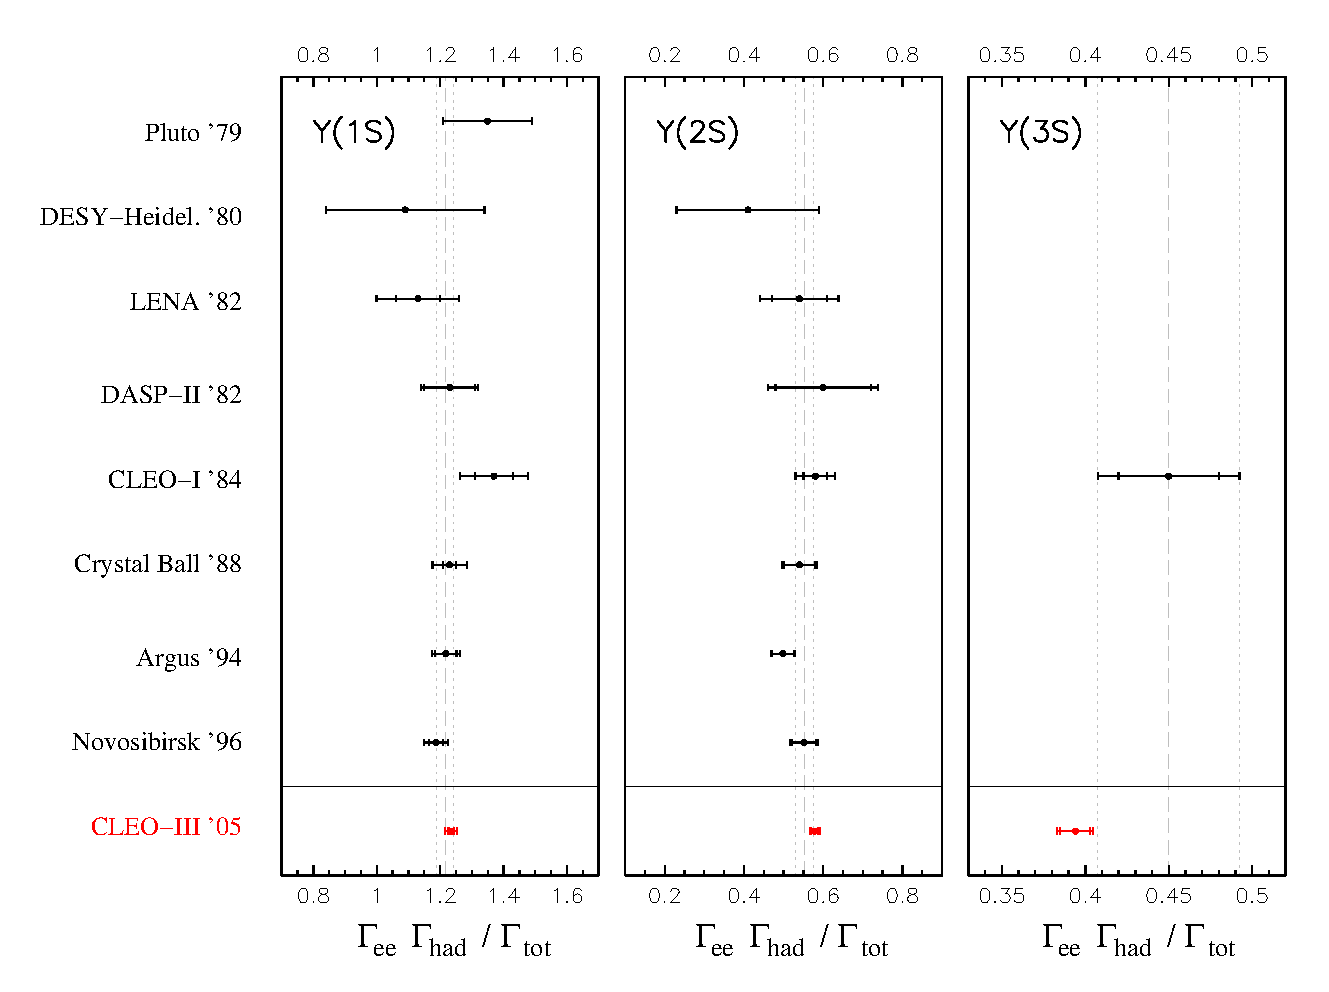
\includegraphics[width=0.95\linewidth]{pdgplots2}
  \end{center}
  \vspace{-1 cm}

\end{slidemap}

%% Comparison with theory (2)

%%   * Theoretical result is incomplete

%%     - Equation 23: missing Z_match is lattice current -> real current
%%       renormalization, and therefore includes discretization
%%       corrections

%%     - For now, we can compare *ratio* of U(2S)/U(1S) with theory

%%     - (Add theory extrapolation to plot and update reference)

%%     - Chiral extrapolation on left, lattice spacing dependence on
%%       right

%%     - \Gamma_ee(1S,2S,3S) calculations will ultimately be ~10%
%%       accurate, but ratios will be few percent

\begin{slidemap}[\mboxy{technique} & \mboxy{backgrounds} & \mboxy{efficiency} & \mboxy{luminosity} & \mboxy{stability} & \mboxy{fits} & \mboxy{results} & \mboxy{\color{blue} \bf theory}]

\vspace{0.4 cm}
\begin{itemize}\setlength{\itemsep}{0.4 cm}

  \item Theoretical result is incomplete--- missing lattice renormalization factor

  \item For now, we can compare {\it ratio} of
  $\Gamma_{ee}(2S)/\Gamma_{ee}(1S)$

  \begin{center}
    \mbox{\hspace{2.7 cm}} Chiral extrapolation \mbox{\hspace{4.7 cm}} Lattice spacing extrapolation \\
    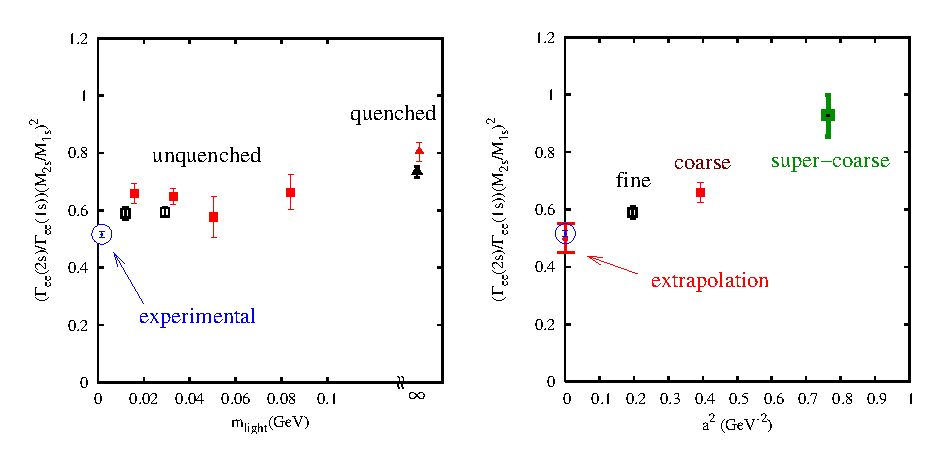
\includegraphics[width=\linewidth]{dependence}
    %% (hep-lat:0507013, 13 July 2005)
  \end{center}

  \item $\Gamma_{ee}(1S,2S,3S)$ calculations will ultimately be
  $\sim$10\% accurate

  \item Ratios will be a few percent

\end{itemize}
\vspace{-0.4 cm}

\end{slidemap}

%% D TO MU NU

%% Similar roadmap (1)

\begin{slidemappy}[\mboxy{introduction} & \mboxy{event selection} & \mboxy{backgrounds} & \mboxy{results}]

\begin{center}
  \begin{minipage}{0.7\linewidth}

    $D^+ \to \mu^+ \nu$ Table of Contents

    \vspace{0.4 cm}
    \begin{center}
      \begin{minipage}{0.95\linewidth}
        \begin{itemize}\setlength{\itemsep}{0.5 cm}

          \item Introduction

          \item Event selection

          \item Backgrounds

          \item Results and comparison with theory

        \end{itemize}
      \end{minipage}
    \end{center}

  \end{minipage}

\end{center}

\end{slidemappy}

%% Introduction (3, really 2)

%%   * Very different kind of analysis: discovery, statistics-limited

%%   * CLEO-c (show cut-away, point out SI -> ZD) with 281 pb^-1 at
%%     psi(3770) (produces D\bar{D} pairs)

%%   * Identify D+ on one side of the event and look for signal:
%%     D- -> mu nu (or charge conjugate)

%%     - Event picture of a typical D- -> mu nu

%%     - Six tag modes, following the MARK-III procedure very closely

\begin{slidemappy}[\mboxy{\color{blue} \bf introduction} & \mboxy{event selection} & \mboxy{backgrounds} & \mboxy{results}]

\vfill

\begin{itemize}

  \item Very different kind of analysis: discovery, statistics-limited

  \item 281 pb$^{-1}$ at $\psi(3770) \to D\bar{D}$

  \item CLEO-III $\to$ CLEO-c: new inner tracker

\end{itemize}

\vfill

\begin{center}
  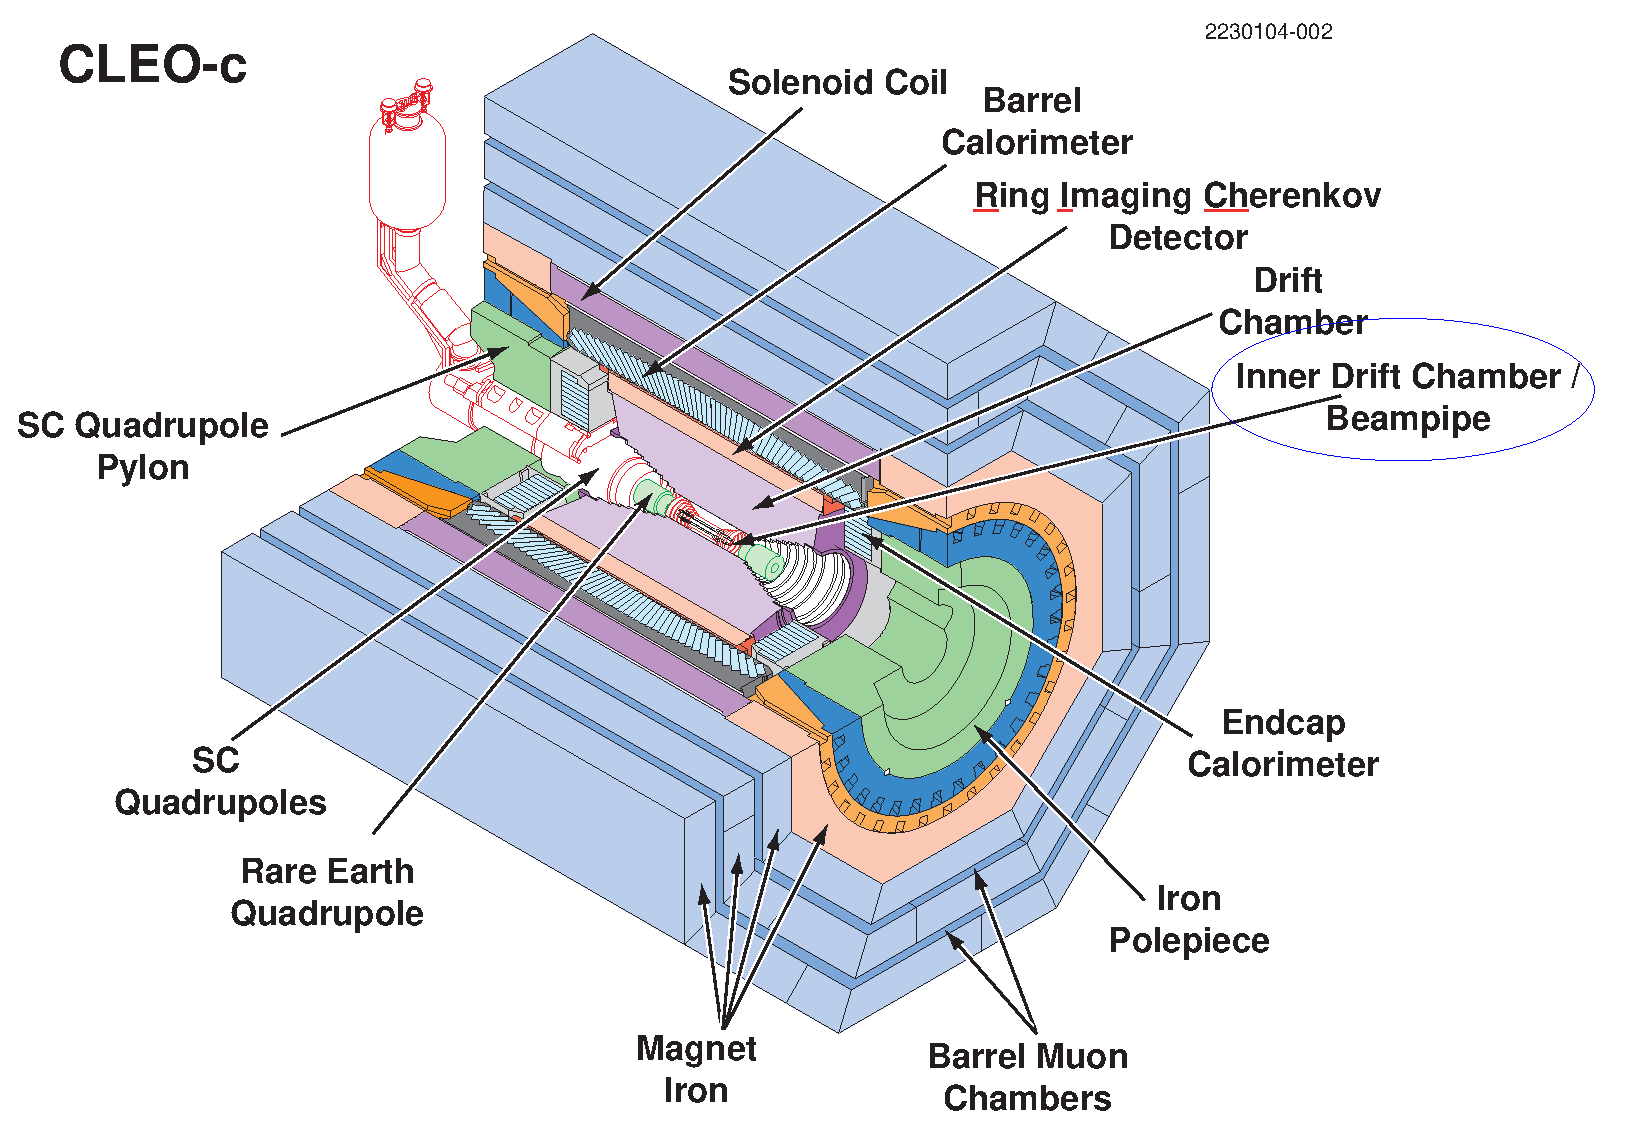
\includegraphics[width=0.7\linewidth]{cleoc_2}
\end{center}

\end{slidemappy}

\begin{slidemappy}[\mboxy{\color{blue} \bf introduction} & \mboxy{event selection} & \mboxy{backgrounds} & \mboxy{results}]

\vfill

\begin{center}
  \begin{tabular}{p{0.6\linewidth} p{0.35\linewidth}}
    \begin{minipage}{\linewidth}
      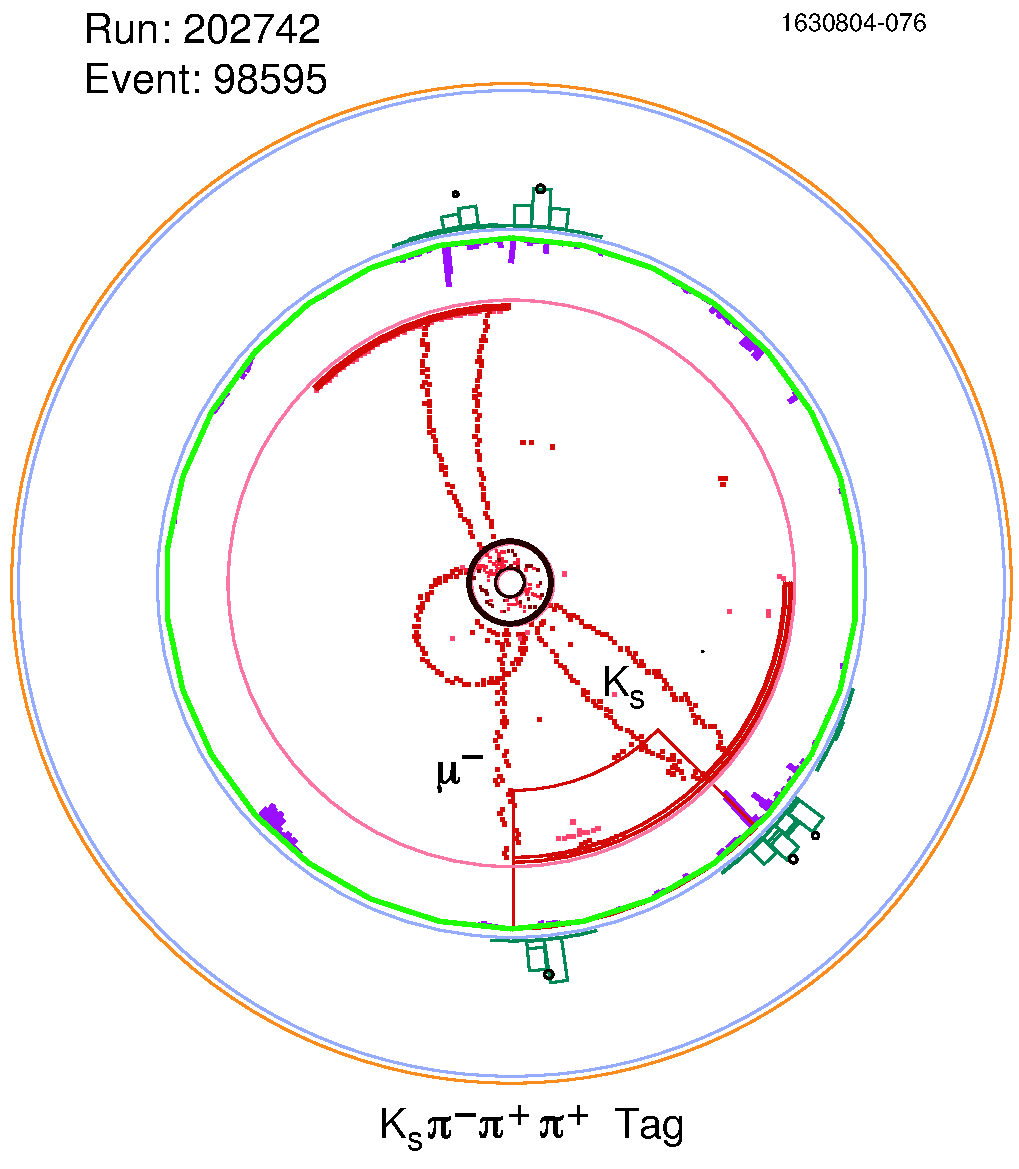
\includegraphics[width=\linewidth]{dmunu_event}
    \end{minipage} &
    \begin{minipage}{\linewidth}
      \begin{itemize}

	\item Follows MARK-III procedure very closely

	\item Fully reconstruct $D^-$ decay on one side and search for
	  $\mu^+ \nu$ signal on the other

      \renewcommand{\arraystretch}{1.25}
      \begin{center}
        \begin{tabular}{l}
  	  Tag Modes \\\hline\hline
  	  $K^+\,\pi^-\,\pi^-$ \\
  	  $K^+\,\pi^-\,\pi^-\,\pi^0$ \\
  	  $K^0_S\,\pi^-$ \\
  	  $K^0_S\,\pi^-\,\pi^-\,\pi^+$ \\
  	  $K^0_S\,\pi^-\,\pi^0$ \\
  	  $K^+\,K^-\,\pi^-$ \\
        \end{tabular}
      \end{center}

      \end{itemize}
    \end{minipage}
  \end{tabular}
\end{center}

\end{slidemappy}

%% Event selection (2)

%%   * Tag modes are fully reconstructed (each track identified,
%%     pions/kaons cleanly distinguished by RICH detector, no
%%     unidentified CsI showers > 250 MeV)

%%     - Plot from updated paper

%%   * Muon deposits < 300 MeV in CsI calorimeter (cuts out 60% of pions)

%%   * Neutrino is reconstructed from missing mass^2 (define)

%%     - Plot from updated paper

%%     - Large peak is from D+ -> K^0 pi, where the K^0 is lost:
%%       0.25 GeV^2 is the mass^2 of the K^0

%%     - D+ -> mu nu (and conjugates) peak near zero (previous
%%       measurement at BES saw 3 events)

\begin{slidemappy}[\mboxy{introduction} & \mboxy{\color{blue} \bf event selection} & \mboxy{backgrounds} & \mboxy{results}]

\begin{center}
  \begin{tabular}{p{0.3\linewidth} c p{0.345\linewidth} c p{0.3\linewidth}}
    \begin{minipage}{\linewidth}
      $\mu/K$ and $\pi/K$ separation
      \begin{itemize}

	\item Energy loss in drift chamber ($dE/dx$)

	\item RICH detector above 0.55 GeV

      \end{itemize}
    \end{minipage} & \mbox{\hspace{0.3 cm}} &
    \begin{minipage}{\linewidth}
      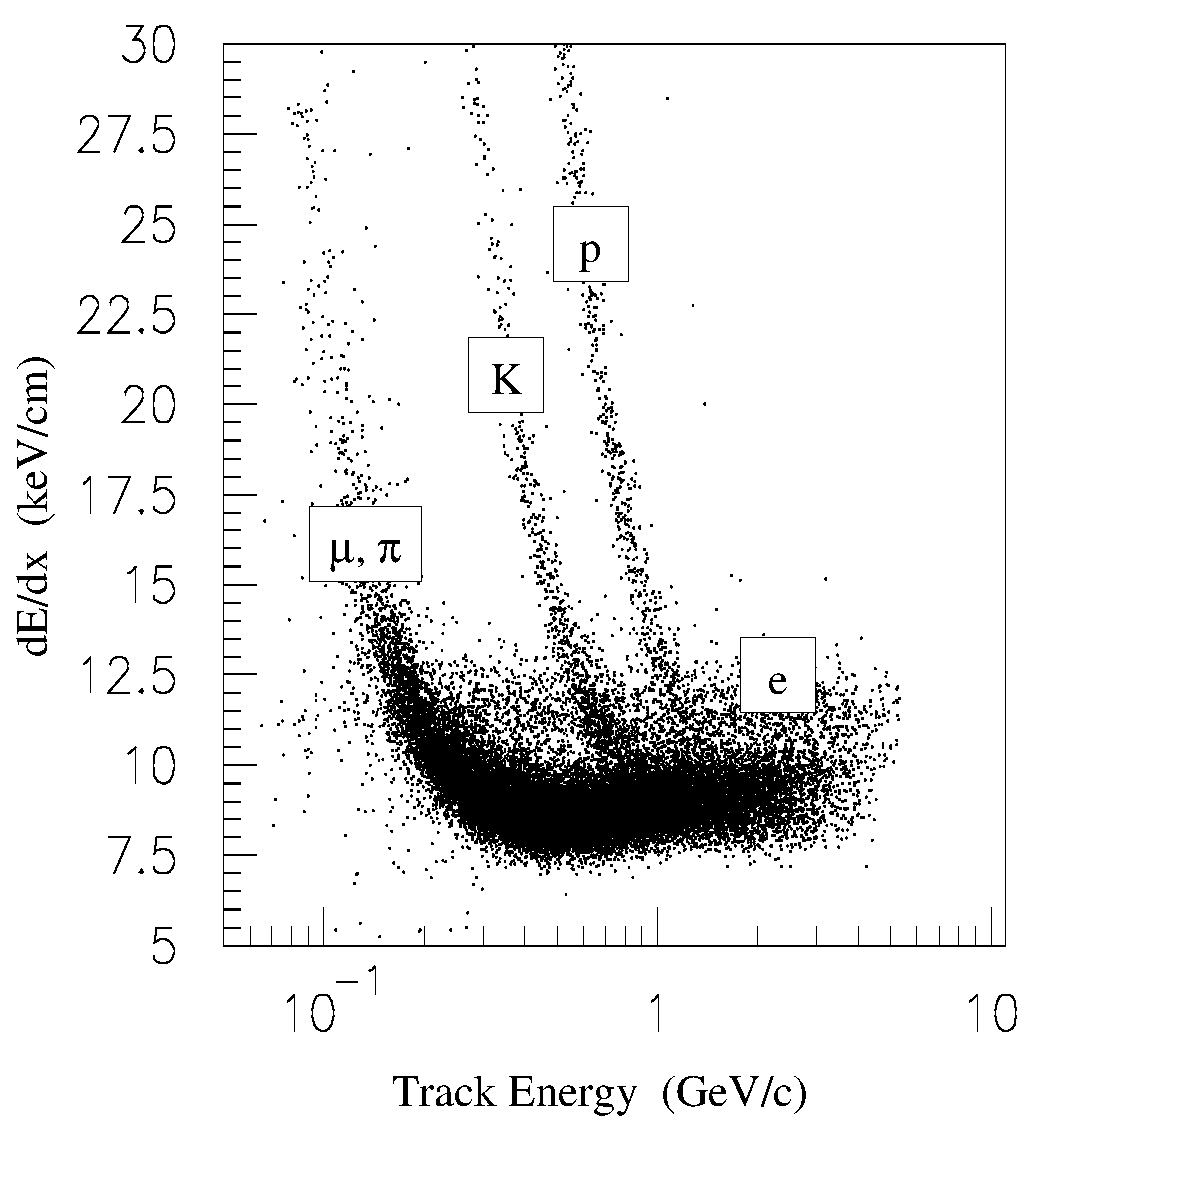
\includegraphics[width=\linewidth]{dedx}
    \end{minipage} & \mbox{\hspace{-1.5 cm}} &
    \begin{minipage}{\linewidth}
      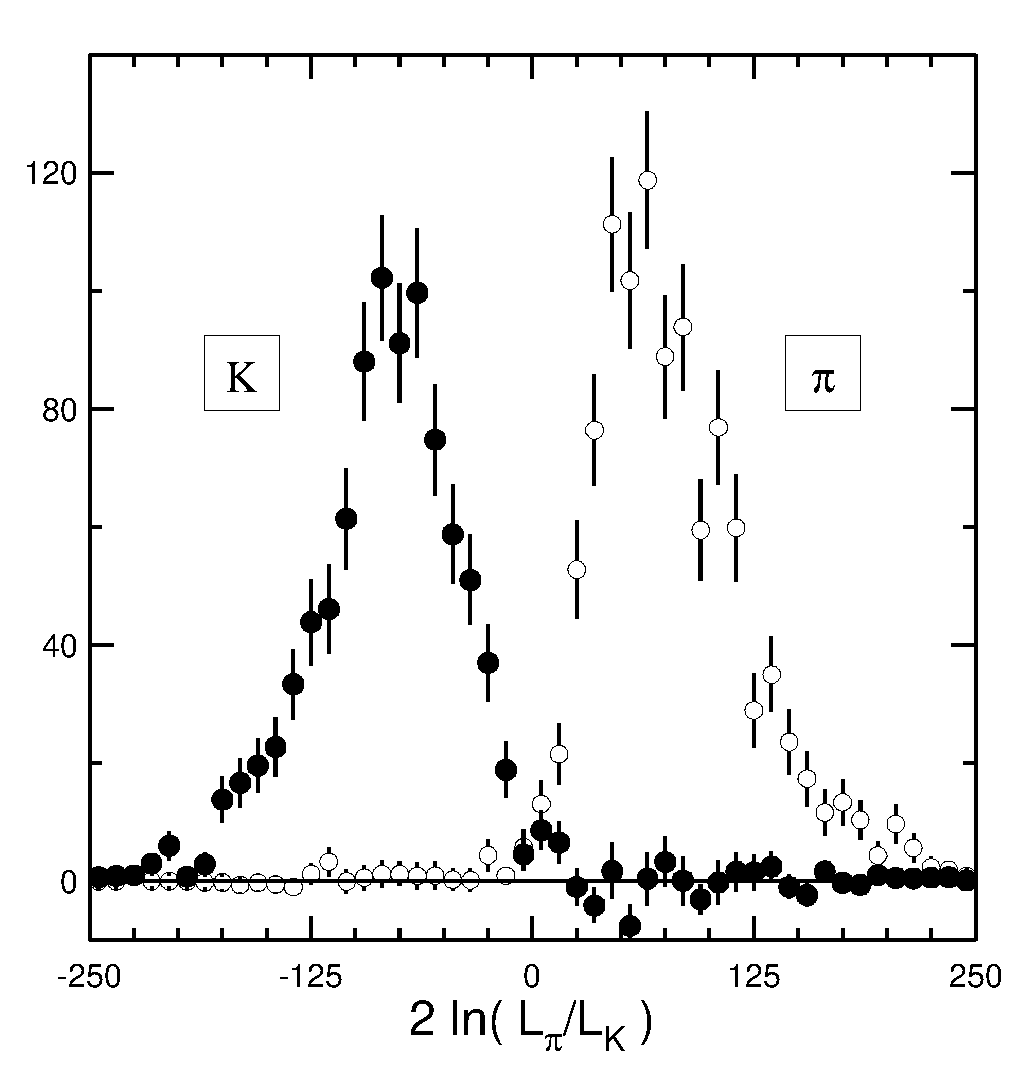
\includegraphics[width=\linewidth]{rich_kpisep2} \vspace{-0.12 cm}
    \end{minipage}
  \end{tabular}

  \vspace{0.5 cm}
  \begin{tabular}{p{0.55\linewidth} c p{0.4\linewidth}}
    \begin{minipage}{\linewidth}
      Beam-constrained mass {\LARGE $m_{BC} = \sqrt{{E_{beam}}^2 - \left|\sum_i \vec{p}_i\right|^2}$}

      \vspace{0.5 cm}
      \begin{itemize}

	\item Background: 3$^{rd}$-order polynomial or \mbox{ARGUS} function

	\item Signal: Gaussian for most modes, double-Gaussian for
	$K^+\,\pi^-\,\pi^-$ and $K^0_S\,\pi^-$

      \end{itemize}


    \end{minipage} & &
    \begin{minipage}{\linewidth}
      \includegraphics[width=\linewidth, clip=true]{dmunu_mbc}
    \end{minipage}
  \end{tabular}
\end{center}

\end{slidemappy}

\begin{slidemappy}[\mboxy{introduction} & \mboxy{\color{blue} \bf event selection} & \mboxy{backgrounds} & \mboxy{results}]

\begin{itemize}

  \item $\mu^+$: track within $|\cos\theta| < 0.81$ pointing to event
  vertex ($\pm$ 5 mm in XY, 5 cm in Z) matched to less than 300 MeV in
  CsI calorimeter

\end{itemize}

\vspace{0.5 cm}

\begin{minipage}{0.35\linewidth}
  \begin{itemize}\setlength{\itemsep}{0.5 cm}
    
    \item $\nu$: missing mass$^2$ within 0.05 GeV$^2$ of zero

    \item 50 events in signal region

    \vspace{10 cm}
    \item $K^0_L$ mass$^2$ is 0.25 GeV$^2$

  \end{itemize}
\end{minipage} \hfill \begin{minipage}{0.6\linewidth}
  \includegraphics[width=\linewidth, clip=true]{dmunu_mm}
\end{minipage}

\hfill $MM^2 = (E_{beam} - E_{\mu^+})^2 - |-\vec{p}_{D^-} - \vec{p}_{\mu^+}|^2$ \hspace{0.3 cm}

\vspace{-1 cm}

\end{slidemappy}

%% Backgrounds (1)

%%   * Table of background contributions (MC) (use updated paper text)

%%     - All background rates are small: 2.8 background / 47.2 signal

\begin{slidemappy}[\mboxy{introduction} & \mboxy{event selection} & \mboxy{\color{blue} \bf backgrounds} & \mboxy{results}]

\vfill

\begin{itemize}\setlength{\itemsep}{0.75 cm}

  \item $D^+ \to K^0_L \pi^+$:

    \vspace{0.1 cm}
    \begin{itemize}\setlength{\itemsep}{0.25 cm}

      \item Identify $D^0 \to K^- \pi^+$ in $D^0\bar{D^0}$ sample

      \item Ignore kaon, and compute missing mass$^2$

      \item Background is 0.3 $\pm$ 0.2 events

    \end{itemize}

  \item $D^+ \to \pi^+ \pi^0$:

    \vspace{0.1 cm}
    \begin{itemize}\setlength{\itemsep}{0.25 cm}

      \item Monte Carlo $+$ branching fractions $\Rightarrow$ background is 1.4 $\pm$ 0.3 events

    \end{itemize}

  \item $D^+ \to \tau^+ \nu$:

    \vspace{0.1 cm}
    \begin{itemize}\setlength{\itemsep}{0.25 cm}

      \item Related to signal

      \item Monte Carlo $+$ branching fractions $\Rightarrow$ background is 1.1 $\pm$ 0.2 events

    \end{itemize}

  \item $D^+ \to$ anything else, $D^0\bar{D^0}$ and continuum backgrounds

    \vspace{0.1 cm}
    \begin{itemize}\setlength{\itemsep}{0.25 cm}

      \item 2.3 fb$^{-1}$ of Monte Carlo (8$\times$ signal) $\Rightarrow$ no events

    \end{itemize}

\end{itemize}

\vfill

Total background is 2.8 $\pm$ 0.4 events $\Rightarrow$ yield of 47.2 $\pm$ 7.1 $^{+0.3}_{-0.8}$ signal events

\end{slidemappy}

%% Systematic uncertainties characterize MC accuracy (table) (1)

%%   * Clean environment, well-understood detector, tested MC
%%     --> 2% systematic

%%   * Statistical uncertainty is 15%

%% Final results (quote paper, make a PDG plot out of the predictions) (1)

\begin{slidemappy}[\mboxy{introduction} & \mboxy{event selection} & \mboxy{backgrounds} & \mboxy{\color{blue} \bf results}]

\vspace{0.5 cm}

\begin{itemize}

  \item Clean environment, well-understood detector $\to$ 2\% systematic uncertainty

  \item Statistical uncertainty is 15\%

  \item $\mathcal{B}(D^+ \to \mu^+\nu)$ = (4.40 $\pm$ 0.66 $^{+0.09}_{-0.12}$) $\times$ 10$^{-4}$ \hfill and \hfill $f_{D^+}$ = (222.6 $\pm$ 16.7 $^{+2.8}_{-3.4}$) MeV

\end{itemize}

\vspace{0.5 cm}

\begin{center}
  \includegraphics[width=0.55\linewidth]{dmunu_comparison2}
\end{center}

\vspace{-1 cm}

\end{slidemappy}

\begin{slide}[\boldmath $\Gamma_{ee}$ without a scan]

\begin{center}
  \includegraphics[width=0.7\linewidth]{psi_gamee2}
\end{center}

\begin{itemize}\setlength{\itemsep}{0.4 cm}

  \item $e^+e^-($3770 MeV$) \to$ {\boldmath \color{purple} $\gamma$}
  $\psi(2S)$ is the primary background to $\psi(3770) \to \pi^+\pi^- J/\psi$

  \item {\color{purple} ISR photon} is not reconstructed, but inferred
  from missing momentum

  \item Equivalent to a scan with exactly one energy point, far above
  resonance mass

  \vspace{0.2 cm}
  \begin{itemize}\setlength{\itemsep}{0.4 cm}

    \item ISR lineshape is convoluted with $\psi(2S)$ BW, so it is
    normalized by BW area

    \item $\pi^+\pi^- J/\psi$ is a particularly sensitive channel for $\psi(2S)$

    \item $\Gamma_{ee}(\psi(2S))$ = 2.13 $\pm$ 0.03 $\pm$ 0.08 keV
    (4\% measurement)

    \item Limited by branching fraction uncertainties

  \end{itemize}

\end{itemize}

\vspace{-1 cm}

\end{slide}

%% FUTURE

%% Return to f_D, f_B, \Gamma_ee table (2)

%%   * Add a dimension: f_Ds (th vs expt), f_Bs (theory only)

%%     - Theory errors cancel in f_Bs/f_B, so measure
%%       \Delta_m_Bs/\Delta_m_B for V_ts/V_td

%%     - CLEO-c will measure f_Ds, and therefore f_Ds/f_D

%%     - LQCD does the same and extrapolates to B meson (in fact, more
%%       errors cancel in "Grinstein ratio": (f_Bs/f_Bd)/(f_Ds/f_D))

%%     - CESR/CLEO is already optimizing an energy point for Ds
%%       production

%%   * Semi-leptonic decays: q^2 dependence of f_D (big diagram)

%%     - Difficult to measure far above threshold (CLEO-III plots)
%%       (K l nu peaks under pi l nu)

%%     - Easier at threshold (pastedGraphic; Fig1-a,b CLNS 05-1906)
%%       (This is only 55.8/281 of the currently available data: work in
%%       progress)

\begin{slide}[Future confrontations between LQCD and experiment at CLEO-c]

\begin{itemize}\setlength{\itemsep}{0.5 cm}

  \item LQCD uncertainties cancel in ratios such as $\displaystyle \frac{f_{B_s} B_{B_s}}{f_B B_B}$

  \item Compare experiment and theory for $f_{D_s}$ as well: $D_s \to \mu \nu$

  \item CLEO-c is already optimizing an energy point for $D_s$ production

  \item Optimal use of LQCD and data: $\displaystyle \frac{f_{B_s}}{f_B} = \left(\frac{f_{B_s} f_D}{f_B f_{D_s}}\right)_{\mbox{\large LQCD}} \ \left(\frac{f_{D_s}}{f_D}\right)_{\mbox{\large experiment}}$

\end{itemize}

\begin{center}
  \includegraphics[width=0.5\linewidth]{diagram_semileptonic}
\end{center}

\end{slide}

\begin{slide}[Future confrontations between LQCD and experiment at CLEO-c]

  stuff about semileptonics

\end{slide}

%% SUMMARY (1)

%%   * Precision LQCD is a breakthrough in its own right

%%   * As a tool, it can extract fundumental parameters from decay rate
%%     measurements

%%   * Some contacts with experiment, such as \Gamma_ee, f_D, f_Ds, f(q^2)
%%     Can use these to

%%     - Check the validity the calculations in different quark pair
%%       settings

%%     - Extrapolate experimental measurements, such as f_D and f_Ds/f_D,
%%       to higher quark masses

\begin{slide}[Summary (I haven't proofread this)]

\vspace{0.5 cm}
\begin{itemize}\setlength{\itemsep}{0.5 cm}

  \item Precision LQCD is a breakthrough in its own right

  \item As a tool, it can extract fundumental parameters from decay rate
    measurements

  \item Some contacts with experiment, such as $\Gamma_{ee}$, $f_D$, $f_{Ds}$, $f(q^2)$
    Can use these to

    \vspace{0.3 cm}
    \begin{itemize}\setlength{\itemsep}{0.5 cm}

      \item Check the validity the calculations in different quark pair
      settings

      \item Extrapolate experimental measurements, such as $f_D$ and $f_{Ds}/f_D$,
      to higher quark masses

    \end{itemize}

\end{itemize}

\end{slide}

\end{document}
